%%%%%%%%%%%%%%%%%%%%%%%%%%%%%%%%%%%%%%%%%
% PESTI Report Class File 
%
% Adapted to PESTI/ISEP style (April/2024) by 
%  Elsa Ferreira Gomes (efg@isep.ipp.pt) and 
%  Jorge Coelho (jmn@isep.ipp.pt)
%%%%%%%%%%%%%%%%%%%%%%%%%%%%%%%%%%%%%%%%%%%%
% TMDEI Dissertation
% LaTeX Template
% Version 0.1 (Dec/2015)
%
% Adapted to TMDEI/ISEP style (Dec/2015) by
%  Nuno Pereira (nap@isep.ipp.pt) and
%  Paulo Baltarejo (pbs@isep.ipp.pt)
%
% Based on MastersDoctoralThesis Version 1.2 by Vel (vel@latextemplates.com) and
% Johannes Böttcher, downloaded from (21/11/15):
% http://www.LaTeXTemplates.com
%
% This template is originally based on a template by:
% Steve Gunn (http://users.ecs.soton.ac.uk/srg/softwaretools/document/templates/)
% Sunil Patel (http://www.sunilpatel.co.uk/thesis-template/)
%
% Template license:
% CC BY-NC-SA 3.0 (http://creativecommons.org/licenses/by-nc-sa/3.0/)
%
%%%%%%%%%%%%%%%%%%%%%%%%%%%%%%%%%%%%%%%%%
%https://www.overleaf.com/project/5bfd7e508cfbf932785021c9
%----------------------------------------------------------------------------------------
%	PACKAGES AND OTHER DOCUMENT CONFIGURATIONS
%----------------------------------------------------------------------------------------

\documentclass[
11pt, % The default document font size, options: 10pt, 11pt, 12pt
%oneside, % Two side (alternating margins) for binding by default, uncomment to switch to one side (for drafting/reading purposes)
%english, % english for English;
portuguese,% for Portuguese; delete temporary files if you change language (e.g. 'make clean; make')
singlespacing, % Single line spacing, alternatives: onehalfspacing or doublespacing (for drafting/reading purposes)
%draft, % Uncomment to enable draft mode (no pictures, no links, overfull hboxes indicated)
%nolistspacing, % If the document is onehalfspacing or doublespacing, uncomment this to set spacing in lists to single
liststotoc, % Uncomment to add the list of figures/tables/etc to the table of contents (recommended)
%toctotoc, % Uncomment to add the main table of contents to the table of contents (not recommended)
parskip, % Add space between paragraphs (recommended)
%nohyperref, % Uncomment to not load the hyperref package (not recommended)
nohyperreflinkcolor, % hyperref links are not colored (comment to color links, for example to produce an electronic-only version)
headsepline, % Uncomment to get a line under the header
]{PESTI-style} % The class file specifying the document structure


\usepackage[table]{xcolor}
\usepackage{array}

\usepackage{tikz}
 
\usepackage{pgfplots} % Required for drawing high--quality function plots (can be removed if not used)
\pgfplotsset{compat=newest}

%
% Next you have examples of admissable citation styles; we recomend using the authoryear-comp citation style (which resembles Harvard); don't forget to only uncomment one
%

% authoryear-comp: recommended citation style (e.g. (Buendía, 1860), (Buendía 1910, Arcadio 1940))
\usepackage[style=authoryear-comp,backend=biber]{biblatex} % Bibtex backend with the authoryear-comp citation style (authoryear citations, bibliography ordered alphabetically)

% numeric citation style (e.g. [1], [1-3])
%\usepackage[style=numeric-comp,sorting=none,backend=biber]{biblatex} % Bibtex backend with the numeric-comp citation style (numeric citations, bibliography ordered by appearance)

% alphabetic citation style (e.g. [Buendía10], [Buendía10, Arcadio40])
%\usepackage[style=alphabetic,sorting=none,backend=biber]{biblatex} % Bibtex backend with the alphabetic citation style (alphabetic citations, bibliography ordered by appearance)
  
\addbibresource{mainbibliography.bib} % The filename of the bibliography
 
\makeglossaries % build the glossary
 
% %----------------------------------------------------------------------------------------
% %	THESIS INFORMATION
% %----------------------------------------------------------------------------------------

\thesistitle{{[}Painel ESG - Gestão Sustentável{]}} % Your thesis title, this is used in the title, print it elsewhere with \ttitle

\thesissubtitle{{[}DevScope - Devscope SA{]}} % Your thesis title, this is used in the title, print it elsewhere with \tsubtitle

\thesisdate{2024/2025}
%\author{Nome do Candidato e \textsc{Sobrenome}} % Your name, this is used in the title page, print it elsewhere with \authorname

\author{1220683 | Matilde Varela}

\subjectarea{Computer Systems} % Specialisation area (Computer Systems, Information and Knowledge Systems, Graphics, Systems and Multimedia, Software Engineering), used in the title page, print it elsewhere with \areaname

\supervisor{Paulo Rogério Soares Proença}
\cosupervisor{David Mota}
%\supervisor{Nome \textsc{Sobrenome}} % Your supervisor's name, this is used in the title page, print it elsewhere with \supname

\university{Instituto Superior de Engenharia do Porto}

\monthyear{Julho 2025}

\keywords{Keyword1, ..., Keyword6} % Please define up to 6 keywords that better describe your work, print it elsewhere with \keywordnames

\university{\href{https://www.isep.ipp.pt/}{Instituto Superior de Engenharia do Porto}} % Your university's name and URL, this is used in the title page and abstract, print it elsewhere with \univname

\department{\href{https://www.dei.isep.ipp.pt/}{Departmento de Informática}} % Your department's name and URL, this is used in the title page and abstract, print it elsewhere with \deptname

\thesisdate{Porto, \today} % thesis date,  print it elsewhere with \tdate

% \hypersetup{painel_esg_gestao_sustentavel=\ttitle} % Set the PDF's title to your title
% \hypersetup{matilde_varela=\authorname} % Set the PDF's author to your name
% \hypersetup{pdfkeywords=\keywordnames} % Set the PDF's keywords to your keywords

\begin{document}

%----------------------------------------------------------------------------------------
%	FRONT MATTER
%----------------------------------------------------------------------------------------

% Include the frontmatter of your thesis here
% we include the glossary here (frontmatter is included with \input, so this command is as if it was in main.tex)
\newacronym{ESG}{ESG}{Environmental, Social, and Governance }
\newacronym{GRI}{GRI}{Global Reporting Initiative}
\newacronym{SASB}{SASB}{Sustainability Accounting Standards Board}
\newacronym{ONU}{ONU}{Organização das Nações Unidas}
\newacronym{PESTI}{PESTI}{Projecto / Estágio}
\newacronym{PRI}{PRI}{Princípios para Investimento Responsável}
\newacronym{CRS}{CRS}{Corporate Social Responsibility}
\newacronym{PNL}{PNL}{Processamento de Linguagem Natural}
\newacronym{IA}{IA}{Inteligência Artificial}
\newacronym{ODS}{ODS}{Objetivos de Desenvolvimento Sustentável}
\newacronym{UNEP FI}{UNEP FI}{UNEP Finance Initiative}

\frontmatter % Use roman page numbering style (i, ii, iii, iv...) for the pre-content pages

\pagestyle{plain} % Default to the plain heading style until the thesis style is called for the body content

%----------------------------------------------------------------------------------------
%	TITLE PAGE
%----------------------------------------------------------------------------------------

\maketitlepage


%----------------------------------------------------------------------------------------
%	STATEMENT of INTEGRITY
%----------------------------------------------------------------------------------------
\integritystatement

%----------------------------------------------------------------------------------------
%	DEDICATION  (optional)
%----------------------------------------------------------------------------------------
%
\begin{dedicatory}
Dedico este projeto a todos que me permitiram chegar a este capítulo da minha vida académica.
\end{dedicatory}

%----------------------------------------------------------------------------------------
%	ACKNOWLEDGEMENTS (optional)
%----------------------------------------------------------------------------------------

\begin{acknowledgements}

Gostaria de iniciar esta secção do relatório a expressar a minha profunda gratidão às pessoas que me acompanharam ao longo deste percurso e contribuíram para a conceção deste projeto.

Em primeiro lugar, um sincero agradecimento ao professor Paulo Proença, cujo papel como orientador foi fundamental. A sua disponibilidade para rever o relatório inúmeras vezes permitiu-me apresentar uma versão mais refinada e estruturada deste trabalho.

Agradeço também ao David Mota, supervisor dos estágios na Devscope, a quem tive o prazer de conhecer na edição de \textit{FallStack} 2024. Foi ele quem me selecionou para este estágio e acolheu os meus interesses em áreas específicas da informática, que mais tarde se integrariam na minha proposta de estágio.

Um agradecimento especial ao meu \textit{buddy}, André Reis, pela orientação técnica e apoio especializado ao longo do projeto.

A todos os estagiários da Devscope, expresso a minha gratidão por tornarem esta experiência mais acolhedora e enriquecedora.

Quero também agradecer aos meus colegas de universidade, Rita Barbosa, Ana Guterres e Afonso Santos, que sempre me incentivaram e apoiaram durante a licenciatura. A sua amizade e motivação foram essenciais para o meu desenvolvimento académico e profissional.

Um agradecimento à Direção Geral de Ensino Superior, pelo apoio financeiro concedido através da bolsa de estudo durante os três anos da licenciatura, e à Câmara Municipal de Portimão, pelo apoio adicional durante dois anos. O contributo destas instituições foi crucial para que eu pudesse prosseguir os meus estudos.

Por fim, e com um carinho especial, quero agradecer aos meus pais, que, apesar dos desafios e dificuldades, sempre se esforçaram para que eu tivesse acesso ao ensino superior. Agradeço também ao meu namorado e à sua família, que têm sido um pilar fundamental de apoio para esta menina deslocada de casa.
\end{acknowledgements}

%----------------------------------------------------------------------------------------
%	ABSTRACT PAGE
%----------------------------------------------------------------------------------------

\chapter*{\textbf{Resumo}}


Os temas ESG (\textit{Environment}, \textit{Social} e \textit{Governance}) têm vindo a ganhar relevância nos últimos vinte anos, sobretudo no que respeita à divulgação de dados empresariais associados a estes domínios e às suas implicações. A questão do \textit{greenwashing}, as discrepâncias nas classificações ESG fornecidas por várias agências, as abordagens para reduzir o impacto das empresas nestas dimensões e os avanços tecnológicos associados são, atualmente, temas de grande relevância. Este projeto visou a criação de um protótipo de aplicação que permite monitorizar o desempenho ESG de uma empresa.

O presente relatório, elaborado no âmbito da unidade curricular Projeto/Estágio do curso de Licenciatura em Engenharia Informática do Instituto Superior de Engenharia do Porto, apresenta o processo de desenvolvimento da plataforma ESG, realizado para a empresa Devscope, entidade responsável pela orientação do projeto. A ferramenta permite que as organizações carreguem conjuntos de dados, avaliem o desempenho ao nível ESG de várias formas, façam corresponder métricas específicas ao seu contexto, misturem métricas com base na estrutura SASB e estabeleçam objetivos em relação às mesmas métricas.

O desenvolvimento do projeto baseou-se em várias etapas. A primeira fase consistiu na análise do estado da arte, na qual se estuda o conceito de ESG e as suas implicações. Seguiu-se o processo de engenharia de \textit{software}, na qual se procedeu à recolha e análise de requisitos, tanto funcionais como não funcionais. Com os requisitos delineados, procedeu-se à conceção do sistema, definindo a sua arquitetura com base nos modelos C4 e 4+1, bem como as suas funções. Por fim, foram efetuadas as fases de implementação e teste, bem como as evidências e a avaliação geral do que foi feito.

A solução criada cumpre os requisitos e objectivos definidos e é uma aplicação funciona como um \textit{hub} centralizado de apoio à gestão e visualização de temas aplicáveis à ESG para a Devscope. \\

\textbf{Palavras-chave (Tema):}	ESG (\textit{Environment, Social, Governance}), Métricas, Matriz de Materialidade, SASB (\textit{Sustainability Accounting Standards Board}), Conjuntos de Dados \\

\textbf{Palavras-chave (Tecnologias):} React, Next.js, ApexCharts, Railway, AWS S3, Jest

\vspace{20mm}


\begin{abstractotherlanguage}

ESG issues (Environment, Social and Governance) have become increasingly important over the last twenty years, especially with regard to the disclosure of corporate data associated with these areas and their implications. The issue of greenwashing, discrepancies in ESG classifications provided by various agencies, approaches to reducing the impact of companies in these dimensions and the associated technological advances are currently highly relevant topics. This project aimed to create a prototype application to monitor a company's ESG performance.

This report, produced as part of the Project/Internship course of the Degree in Computer Engineering at the Instituto Superior de Engenharia do Porto, presents the process of developing the ESG platform for the company Devscope, the organisation responsible for guiding the project. The tool allows organisations to upload data sets, assess performance at ESG level in various ways, match specific metrics to their context, mix metrics based on the SASB framework and set objectives in relation to the same metrics.

The project was developed in several stages. The first stage consisted of analysing the state of the art, studying the concept of ESG and its implications. This was followed by the software engineering process, in which both functional and non-functional requirements were collected and analysed. Once the requirements had been outlined, the system was designed, defining its architecture based on the C4 and 4+1 models, as well as its functions. Finally, the implementation and testing phases were carried out, as well as the evidence and general evaluation of what had been done.

The solution created meets the requirements and objectives defined and is an application that functions as a centralised hub to support the management and visualisation of ESG issues for Devscope. \\

\textbf{Keywords (Theme):}	ESG (Environment, Social, Governance), Metrics, Materiality Matrix, SASB (Sustainability Accounting Standards Board), Data Sets \\

\textbf{Keywords (Technologies):} React, Next.js, ApexCharts, Railway, AWS S3, Jest

\end{abstractotherlanguage}


%----------------------------------------------------------------------------------------
%	LIST OF CONTENTS/FIGURES/TABLES PAGES
%----------------------------------------------------------------------------------------

\tableofcontents % Prints the main table of contents

\listoffigures % Prints the list of figures

\listoftables % Prints the list of tables

% \iflanguage{portuguese}{
% \renewcommand{\listalgorithmname}{Lista de Algor\'itmos}
% }
% \listofalgorithms % Prints the list of algorithms
% \addchaptertocentry{\listalgorithmname}


\renewcommand{\lstlistlistingname}{List of Source Code}
\iflanguage{portuguese}{
\renewcommand{\lstlistlistingname}{Lista de C\'odigo}
}

\lstlistoflistings
\addcontentsline{toc}{chapter}{\lstlistlistingname}


%----------------------------------------------------------------------------------------
%	ABBREVIATIONS
%----------------------------------------------------------------------------------------
% \begin{abbreviations}{ll} % Include a list of abbreviations (a table of two columns)
% \begin{table}[h]
%     \centering
%     \begin{tabular}{|c|c|}
%         \hline
%         \textbf{ESG} & \textbf{E}nvironmental, \textbf{S}ocial and \textbf{G}overnance \\ \hline
%         \textbf{SASB} & \textbf{S}ustainability, \textbf{A}ccounting \textbf{S}tandards \textbf{B}oard \\ \hline
%         \textbf{GRI} & \textbf{G}lobal, \textbf{R}eporting \textbf{I}nitiative \\ \hline
%     \end{tabular}
% \end{table}
% \end{abbreviations}

%----------------------------------------------------------------------------------------
%	SYMBOLS
%----------------------------------------------------------------------------------------

% \begin{symbols}{lll} % Include a list of Symbols (a three column table)

% $a$ & distance & \si{\meter} \\
% $P$ & power & \si{\watt} (\si{\joule\per\second}) \\
% %Symbol & Name & Unit \\

% \addlinespace % Gap to separate the Roman symbols from the Greek

% $\omega$ & angular frequency & \si{\radian} \\

% \end{symbols}

%----------------------------------------------------------------------------------------
%	ACRONYMS
%----------------------------------------------------------------------------------------

% \newcommand{\listacronymname}{List of Acronyms}
% \iflanguage{portuguese}{
% 	\renewcommand{\listacronymname}{Lista de Acr\'onimos}
% }

% %Use GLS
% \glsresetall
% \printglossary[title=\listacronymname,type=\acronymtype,style=long]
% \addcontentsline{toc}{chapter}{\listacronymname}


\begin{acronyms}{lp{4cm}p{10cm}} % Adjust column widths as needed
\textbf{Sigla} & \textbf{Definição} \\ \midrule
API & Application Programming Interface \\
CRS & Corporate Social Responsibility \\
ESG & Environmental, Social, and Governance \\
GEE & Gases de Efeito Estufa \\
GRI & Global Reporting Initiative \\
HTML & HyperText Markup Language \\
HTTP & HyperText Transfer Protocol \\
IA & Inteligência Artificial \\
ISEP & Instituto Superior de Engenharia do Porto \\
IoT & Internet of Things \\
IT & Information Technology \\
JSON & JavaScript Object Notation \\
KPI & Key Performance Indicator \\
LEI & Licenciatura em Engenharia Informática \\
ODS & Objetivos de Desenvolvimento Sustentável \\
ONU & Organização das Nações Unidas \\
PESTI & Projecto / Estágio \\
PNL & Processamento de Linguagem Natural \\
PRI & Princípios para Investimento Responsável \\
RFID & Radio-Frequency Identification \\
SaaS & Software as a Service \\
SASB & Sustainability Accounting Standards Board \\
SPA & Single Page Application \\
UI & User Interface \\
UNEP FI & UNEP Finance Initiative \\
URL & Uniform Resource Locator \\
\end{acronyms}


%----------------------------------------------------------------------------------------
%	DONE
%----------------------------------------------------------------------------------------

\mainmatter % Begin numeric (1,2,3...) page numbering
\pagestyle{thesis} % Return the page headers back to the "thesis" style


%----------------------------------------------------------------------------------------
%	MAIN BODY
%----------------------------------------------------------------------------------------

% Include the chapters of the thesis as separate folder for each chapter
% Uncomment the lines as you write the chapters

% % Chapter 1
% 
\chapter{Introdução} % Main chapter title
\label{chap:Introdução} % For referencing the chapter elsewhere, use Chapter~\ref{Introdução}


% \textbf{Nota: devem usar frases curtas; adotar o impessoal em vez do pessoal (e.g. adotou-se vs. adotei vs. adotamos); usar verbos conjugados no presente; evitar encadear verbos seguidos (e.g. “esta secção vai ser descrito” vs. “esta secção descreve”); usar voz passiva vs. ativa.}

% * prespetiva geral do problema de estudo (enquadramento) 

% * problema em estudo e objetivos
% * principais metodos de trabalho usados
% * contributos e aspetos inovadores da soluçao

% * apresentaçao da estrutura/secçoes do relatorio


% \hline


Esta secção tem como objetivo apresentar o projeto, o trabalho realizado e a sua contextualização, abordando o problema em estudo e os objetivos a serem alcançados. Também será feita uma descrição dos principais métodos utilizados ao longo do trabalho, bem como a identificação dos contributos e dos aspetos inovadores da solução desenvolvida. O capítulo conclui com a apresentação da estrutura do presente relatório.


%-------------------------------------------------------------------------------
%---------
%
\section{Enquadramento/Contexto} 
\label{sec:chap1_introduction} %For referencing this section elsewhere, use Section~\ref{sec:chap1_introduction}

Este projeto é um dos elementos mais importantes do curso, integrado na unidade curricular \gls{PESTI}. Através dele, é atribuído um problema a ser resolvido, esperando-se uma solução documentada neste relatório. O principal objetivo deste projeto é desenvolver competências pessoais e profissionais, aplicando os conhecimentos adquiridos ao longo da licenciatura e preparando o estudante para a inserção no mercado de trabalho.

O presente projeto foi desenvolvido durante um estágio em ambiente empresarial na DevScope, uma empresa sediada no Porto, fundada em 2003, com mais de vinte anos de experiência em consultoria e desenvolvimento de \textit{software}. A empresa especializa-se em tecnologias da Microsoft, nomeadamente \textit{Power Platform}, \textit{Portals} (Office 365 \& SharePoint), \textit{Web \& App Development}, \textit{AI \& Machine Learning}, \textit{Business Intelligence}, \textit{Enterprise Integration}, \textit{Cloud \& DevOps} e \textit{Training \& Education} (\cite{DevScopeSolutions}). Os seus serviços são aplicados em diversas áreas, incluindo saúde, retalho e setor imobiliário.

Como parte do programa de estágio, a DevScope proporciona um período inicial de três semanas, denominado Ramp Up, onde os estagiários participam em \textit{workshops} sobre diferentes tecnologias utilizadas na empresa. Este processo acelera a integração dos estagiários nos projetos, reduzindo o tempo necessário para a implementação de soluções. Além disso, a empresa oferece um horário de trabalho remoto e flexível, bem como diversas atividades ao longo do ano, promovendo um ambiente colaborativo e fortalecendo a cultura organizacional.

Nos últimos anos, as empresas têm demonstrado uma preocupação crescente com questões ambientais, sociais e de governança (ESG). Este foco tem levado as organizações a recolher e analisar dados que auxiliem numa tomada de decisão mais consciente e estratégica. No entanto, a falta de centralização no tratamento e visualização desses dados pode comprometer a performance empresarial e expô-la a riscos, como falhas de conformidade regulatória ou problemas éticos.

Assim, torna-se fundamental dispor de uma plataforma que compile e organize estes dados de forma acessível e estruturada, permitindo às empresas obter insights mais claros e estratégicos sobre as suas iniciativas ESG.

O presente projeto tem como objetivo o desenvolvimento do \textit{frontend} desta plataforma, funcionando como o primeiro passo para a criação de uma ferramenta interna da DevScope. Além de contribuir para o desenvolvimento de um protótipo funcional, o projeto permite ao estudante aprender e aplicar ferramentas e tecnologias não abordadas no currículo académico, enriquecendo assim as suas competências técnicas e práticas.


\section{Descrição do Problema}

Nos últimos anos, a DevScope tem vindo a crescer exponencialmente, passando de uma empresa com um ambiente mais familiar para uma estrutura de maior dimensão. Com esse crescimento, surgiu a necessidade de uma plataforma que permita monitorizar e gerir de forma estruturada as iniciativas de \gls{ESG}.

Atualmente, a empresa enfrenta desafios na centralização e análise de métricas ESG, dificultando a identificação de padrões e a tomada de decisões informadas. Questões como consumo de eletricidade, temperatura do escritório e outras métricas ambientais, assim como indicadores sociais e de governança, precisam de ser monitorizados de forma mais acessível e eficiente.

A implementação desta plataforma permitirá um acompanhamento mais estruturado das métricas ESG, facilitando auditorias, identificando comportamentos que possam gerar custos desnecessários e garantindo uma maior transparência. Sem uma solução eficaz, a empresa pode enfrentar perdas financeiras devido a desperdícios operacionais, além de possíveis riscos reputacionais e regulatórios caso não consiga demonstrar conformidade com boas práticas ESG.

O projeto visa desenvolver a interface do utilizador para esta plataforma, garantindo uma experiência intuitiva e eficiente na visualização e gestão dos dados ESG, utilizando frameworks reconhecidos como GRI e SASB para a definição das métricas.


\subsection{Objetivos}

O objetivo principal deste projeto é o desenvolvimento de um \textit{frontend} para o protótipo de uma ferramenta interna da DevScope, que visa o acompanhamento de métricas de \gls{ESG}, facilitando uma tomada de decisão mais informada e estruturada.

Aprofundando-se nos objetivos técnicos, o projeto visa:
\begin{itemize}
    \item \textbf{Centralizar dados de diferentes fontes:} Integrar informações de várias origens para garantir uma visão unificada e acessível.
    \item \textbf{Desenvolver um sistema intuitivo de visualização de dados:} Criar uma interface fácil de usar que permita aos utilizadores analisarem e interpretarem rapidamente as métricas ESG.
    \item \textbf{Automatizar a coleta e o processamento de dados:} Melhorar a precisão dos relatórios por meio de um sistema automatizado que reduz erros manuais e aumenta a eficiência.
\end{itemize}


\subsection{Abordagem} 

O desenvolvimento do projeto seguiu uma abordagem \textit{Agile}, caracterizada pela iteratividade do \textit{software} desenvolvido, pela compreensão das prioridades e pela capacidade de introduzir mudanças ao longo do processo. A flexibilidade perante os pedidos do cliente (DevScope) foi um dos principais fatores, promovendo uma comunicação próxima e frequente (\cite{Patel2025}). O projeto fará ainda uso da \textit{agile framework} \textbf{Scrum}, sendo o projeto divido em iterações de uma semana (\textit{sprints}) e diferentes fases, tais como: pré-planeamento do \textit{sprint} (\textit{release backlog} e \textit{sprint goals}), planeamento do sprint/iteração (\textit{sprint backlog}), implementação e demonstração das funcionalidades desenvolvidas (\cite{Cohen2004}).

Além das metodologias mencionadas, foi utilizado o \textbf{Microsoft OneNote}, uma ferramenta adotada pela DevScope como base de conhecimento colaborativa, desenvolvida pelos próprios colaboradores e acessível a toda a empresa. O \textbf{GitHub} foi empregado não apenas como repositório da solução desenvolvida, mas também como \textit{hub} central do projeto, integrando o quadro \textbf{Kanban}. Esta abordagem, alinhada às metodologias ágeis, visa minimizar o tempo ocioso, promover um fluxo de trabalho mais eficiente e garantir um gerenciamento de tarefas estruturado, por meio de cartões detalhados que acompanham o progresso de cada etapa (\cite{Wakode2021Kanban}).

As funções de \textit{product owner} e \textit{scrum master} foram preenchidas por supervisores da empresa.

O estagiário teve flexibilidade horária, mas manteve comunicação contínua com a empresa. As \textbf{reuniões diárias} (\textit{daily stand-ups}, ~30 min) serviram para atualizar a equipa, enquanto as \textbf{reuniões semanais} garantiram acompanhamento mais detalhado com o supervisor, incluindo demonstrações e \textit{feedback} para orientar o desenvolvimento.

\subsection{Contributos} 

A solução desenvolvida oferece à DevScope uma ferramenta que centraliza e processa informação importante e permite todo um conjunto de benefícios, contribuindo para a mesma de diversas formas:
\begin{itemize}
  \item \textbf{Aumento da produtividade:} Facilitar o acesso e análise das métricas ESG, agilizando o processo de tomada de decisões.
  \item \textbf{Tomadas de decisão mais informadas e estruturadas:} Fornecer dados confiáveis e organizados que suportem decisões empresariais baseadas em métricas claras.
  \item \textbf{Economia financeira:} Identificar comportamentos ineficientes que possam gerar custos desnecessários, promovendo maior eficiência.
  \item \textbf{Avaliação contínua de comportamentos empresariais:} Permitir a monitorização constante de práticas ESG, incentivando um comportamento mais responsável e sustentável.
\end{itemize}


\subsection{Planeamento do trabalho}  

O projeto iniciou-se com uma fase de \textit{Ramp Up} de três semanas, durante a qual são realizados \textit{workshops} sobre as tecnologias utilizadas na DevScope. Após essa etapa inicial, o estágio seguiu um cronograma definido pela empresa, dividido em três fases principais: pesquisa e estado da arte, implementação da solução e refinamento do relatório e da solução. A escrita do relatório teve início após o período de \textit{Ramp Up}.

O cronograma do estágio foi organizado da seguinte forma:

\begin{itemize}
    \item \textbf{Ramp Up}: 24 de fevereiro a 14 de março
    \item \textbf{Estado da Arte}: 17 de março a 4 de abril
    \item \textbf{Implementação}: 14 de abril a 9 de maio
    \item \textbf{Refinamento e Revisão}: 19 de maio a 6 de junho
\end{itemize}

Durante o estágio, ocorreram momentos de avaliação chamados \textit{checkpoints}, nos quais os estagiários apresentaram o progresso do projeto para todos os colaboradores da empresa. Estes momentos são essenciais, pois permitiram a obtenção de \textit{feedback} que foi utilizado para aprimorar tanto a solução desenvolvida quanto o relatório. Foram previstos três \textit{checkpoints} principais:

\begin{enumerate}
    \item \textbf{Estado da Arte} – 7 a 11 de abril
    \item \textbf{Prova de Conceito Funcional} – 12 a 16 de maio
    \item \textbf{Apresentação Final do Projeto e Relatório} – 9 a 13 de junho
\end{enumerate}

Embora a submissão do projeto fosse até 30 de junho, a DevScope planeou concluir essa fase entre 16 e 20 de junho.

 No apêndice \ref{AppendixA}, apresenta-se um diagrama de \textit{Gantt} detalhado com o planeamento definido.


\section{Estrutura do relatório}

O presente relatório é composto por cinco capítulos que descrevem o desenvolvimento da solução para a proposta de \gls{PESTI} escolhida.

A \textbf{Introdução} contextualiza o projeto, apresenta o problema e as abordagens adotadas, destaca os contributos para os \textit{stakeholders} e expõe o cronograma.

O \textbf{Estado da Arte} analisa trabalhos e tecnologias relevantes, explorando soluções existentes relacionadas com o problema em questão.

O capítulo de \textbf{Análise e Desenho da Solução} detalha a metodologia, as tecnologias e os algoritmos utilizados, além da modelação da solução e especificação de requisitos.

A \textbf{Implementação da Solução} descreve aspetos técnicos, como \textit{software}, ferramentas e sistemas utilizados, bem como os testes realizados e a avaliação da solução.

Por fim, as \textbf{Conclusões} apresentam um balanço dos resultados obtidos, analisam as limitações encontradas e incluem uma reflexão crítica sobre o trabalho desenvolvido.

\vspace{20mm} 

% \chapter{Estado da Arte}
\label{chap:EA}

O estado da arte refere-se ao conhecimento atual sobre um determinado tema em análise ou estudo. Este capítulo apresenta uma visão geral das origens do termo ESG, destacando os benefícios da adoção destas práticas, os desafios da sua implementação e monitorização, além de discutir o papel da tecnologia na gestão ESG.

Em seguida, é realizada uma análise dos trabalhos relacionados com a temática do projeto, acompanhada de uma compilação das tecnologias já existentes para a avaliação e gestão de métricas ESG.

%-------------------------------------------------------------------------------

\section{ESG - história do conceito e aplicação} 
\label{sec:OESG} 

O conceito de \gls{ESG} surgiu na década de \textbf{1990}, quando a \gls{ONU} passou a adotar uma postura mais aberta em relação ao setor corporativo. Durante esse período, o então Secretário-Geral da ONU, Kofi Annan, lançou as bases da iniciativa que levaria à criação do conceito de ESG. No contexto da missão das Nações Unidas de promover a paz e o desenvolvimento, aliada aos objetivos do setor empresarial de gerar riqueza e prosperidade, a organização começou a estabelecer parcerias estratégicas, reconhecendo o papel fundamental das empresas no avanço desses objetivos (\cite{Pollman2024}).

Em \textbf{1999}, durante o Fórum Econômico Mundial de Davos, Kofi Annan apresentou a proposta \textit{Global Compact} (\cite{Pollman2024}), que se tornou operacional em \textbf{2000}, de interesse mútuo da ONU e do setor corporativo. De acordo com a \gls{ONU}, trata-se de "um apelo às empresas para alinharem as suas estratégias e operações com princípios universais de direitos humanos, trabalho, meio ambiente e combate à corrupção, e tomem medidas que promovam objetivos sociais" (\cite{ONUGC2025}). Esta iniciativa tem por base dez princípios fundamentados nos direitos humanos, trabalho, meio ambiente e combate à corrupção \footnote{Os princípios que constituem a iniciativa \textit{Global Compact} estão disponíveis no site oficial \textit{UN Global Compact}: \url{https://unglobalcompact.org/what-is-gc/mission/principles} (acesso a 31/03/2025).}.

\subsection{Who Cares Wins}
\label{subsec: WCW}

Em \textbf{2004}, Kofi Annan convidou algumas das principais instituições financeiras do mundo para se unirem à \gls{ONU} numa nova iniciativa, como extensão do \textit{Global Compact}: o projeto \textit{Who Cares Wins}.

Esta iniciativa reuniu, pela primeira vez, investidores institucionais, gestores de ativos, analistas de pesquisa buy-side\footnote{Buy-side refere-se a instituições que compram ativos para investimento próprio, como fundos de investimento e seguradoras.} e sell-side\footnote{Sell-side refere-se a instituições que vendem ativos e oferecem recomendações de investimento, como corretoras e bancos de investimento.}, consultores globais, órgãos governamentais e reguladores, com o objetivo de examinar o papel dos fatores \gls{ESG} na gestão de ativos e na pesquisa financeira (\cite{Pollman2024}).

Como resultado, chegou-se a um consenso sobre o impacto dos fatores ESG no contexto de investimentos de longo prazo, e foi elaborado um relatório\footnote{Uma versão em PDF do relatório de 2004 está disponível em \url{https://www.ifc.org/content/dam/ifc/doc/mgrt/whocareswins-2005conferencereport.pdf} (acesso a 31/03/2025).}, no qual o termo "ESG" foi introduzido oficialmente. O documento também apresentou recomendações para diferentes atores do mercado sobre como integrar questões ambientais, sociais e de governança corporativa na gestão de ativos, nos serviços de corretagem de valores mobiliários\footnote{Corretagem de valores mobiliários refere-se à intermediação na compra e venda de ativos financeiros, normalmente realizada por corretoras.} e nas funções de pesquisa associadas (\cite{onValues2005}).

\begin{figure}[h]
    \centering
    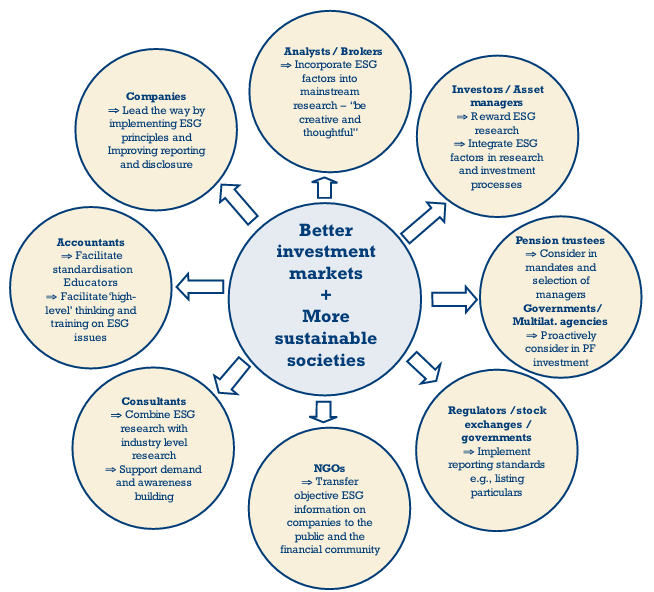
\includegraphics[width=5in]{frontmatter/assets/agentes-chave-esg-wcw.png}
    \caption{Principais intervenientes envolvidos na integração de temáticas ESG segundo o relatório \textit{Who Cares Wins} (\cite{onValues2005})}
    \label{fig:wcwactors}
\end{figure}

Segundo \cite{Pollman2024}, "embora o termo ESG tenha sido mencionado em menos de 1\% das conferências de resultados financeiros nos anos seguintes ao relatório \textit{Who Cares Wins}, em 2021 a sua presença cresceu significativamente, sendo citado em quase um quinto dessas conferências. Além disso, um estudo revelou que 72\% dos investidores institucionais passaram a incorporar fatores ESG nas suas estratégias".

\subsection{PRI: Princípios de Investimento Responsável}
\label{subsec: PRI}

Com a crescente conscientização dos problemas ESG, surgiram outras iniciativas, como os \gls{PRI}. O PRI foi iniciado em \textbf{2005} por Kofi Annan, que convidou um grupo internacional de investidores institucionais a desenvolver iniciativas que refletissem a crescente importância das questões ESG nas práticas de investimento (\cite{Kim2022}).

Os PRI mantêm uma forte ligação à \gls{ONU} através dos seus dois parceiros fundadores — o UN Global Compact e a UNEP Finance Initiative (UNEP FI). A iniciativa assenta em seis princípios \footnote{Os seis princípios para investimento responsável podem ser consultados no site oficial: \url{https://www.unpri.org/about-us/what-are-the-principles-for-responsible-investment} (acesso em 31/03/2025).} concebidos para reforçar a relação entre o investimento responsável e o desenvolvimento sustentável, alinhando o trabalho do PRI com os Objetivos de Desenvolvimento Sustentável (ODS)\footnote{As Nações Unidas disponibilizam um website com informações detalhadas sobre os ODS: \url{https://ods.pt/ods/} (acesso em 31/03/2025).} e incentivando os seus signatários a adotar a mesma abordagem (\cite{PRIBlueprint2017}).

No seu website\footnote{O site oficial do PRI disponibiliza informações detalhadas sobre as várias medidas, práticas e desafios ESG. As \textbf{questões ambientais} podem ser consultadas em \url{https://www.unpri.org/sustainability-issues/environmental-social-and-governance-issues/environmental-issues}, as \textbf{questões sociais} em \url{https://www.unpri.org/sustainability-issues/environmental-social-and-governance-issues/social-issues} e as \textbf{questões de governança} em \url{https://www.unpri.org/sustainability-issues/environmental-social-and-governance-issues/governance-issues} (acesso em 31/03/2025).}, os \gls{PRI} enumeram uma vasta gama de desafios, temáticas e externalidades ESG que as empresas devem considerar cada vez mais. Estes desafios abrangem três grandes dimensões:

\begin{itemize}
\item \textbf{Ambiente} – conservação da natureza, transição para uma economia circular, gestão sustentável da água, impactos do fraturamento hidráulico e emissões de metano.
\item \textbf{Sociedade} – promoção da diversidade, equidade e inclusão, bem como condições de trabalho dignas.
\item \textbf{Governança} – justiça tributária, engajamento político responsável, segurança cibernética, remuneração executiva, propósito corporativo, combate à corrupção, proteção de denunciantes e nomeações de diretores.
\end{itemize}

%-------------------------------------------------------------------------------

\section{Trabalhos relacionados} 
\label{sec:TR} 

Esta secção tem como objetivo apresentar o estado da arte sobre ESG, abordando tanto os desafios e impactos desses fatores nas empresas quanto as soluções já desenvolvidas para sua análise e reporte. Para isso, será feita uma revisão de artigos científicos e tecnologias aplicadas ao mercado.  

Primeiramente, serão exploradas as práticas ESG e os seus efeitos no valor, rentabilidade e riscos das empresas, com base em estudos recentes sobre a relação entre desempenho financeiro e fatores ESG. Em seguida, serão analisadas as principais metodologias e abordagens utilizadas para reporte e análise ESG, destacando a diversidade de métricas e frameworks existentes e os desafios relacionados à sua padronização.  

Posteriormente, serão discutidas as tendências atuais, com ênfase no impacto das novas tecnologias, como inteligência artificial e análise de dados em tempo real, na otimização da gestão ESG. A secção também apresentará um levantamento das principais tecnologias disponíveis no mercado, incluindo frameworks de relato ESG e softwares especializados.  

Por fim, será introduzido o contexto tecnológico da solução proposta, destacando as ferramentas e bibliotecas utilizadas no seu desenvolvimento e justificando a escolha dessas tecnologias com base nas necessidades do projeto.

%-------------------------------------------------------------------------------

\subsection{Práticas e Riscos ESG: Impacto no Valor e Rentabilidade das Empresas}
\label{subsec:PESGE}

O movimento por detrás da sigla ESG é bastante complexo, incorporando elementos de responsabilidade social, ambiental e governança corporativa para avaliar empresas. Os fatores de \gls{ESG} são importantes para medir a sustentabilidade dos agentes econômicos e expandem o escopo do desempenho corporativo. Fatores externos, como o mercado e a indústria, e fatores internos, como a estrutura de propriedade e o conselho de administração, influenciam as práticas ESG na criação de valor (\cite{Wang2023}).

Segundo uma análise conduzida por \cite{Whelan2021}, em colaboração com a \textit{Rockefeller Asset Management} e o \textit{NYU Stern Center for Sustainable Business}, examinou-se mais de 1000 estudos publicados entre 2015 e 2020 sobre a relação entre fatores ESG e desempenho financeiro. Os resultados indicaram que 58\% dos estudos identificaram uma relação positiva, 8\% uma relação negativa, 13\% nenhuma relação e 21\% apresentaram resultados mistos. Embora a maioria dos estudos sugira um impacto positivo dos fatores ESG no desempenho financeiro, os autores concluem que os resultados refletem um debate contínuo sobre o tema.

Os estudos que identificaram uma \textbf{relação positiva} entre práticas ESG e desempenho financeiro apontam uma forte correlação entre a qualidade dos relatórios ESG e o valor da empresa. Isso sugere que a transparência, a confiança e a responsabilização dos \textit{stakeholders} exercem uma influência positiva na valorização da empresa (\cite{Aydomu2022}).

Por outro lado, os estudos que encontraram \textbf{efeitos negativos} destacam diferentes fatores. Entre eles, está o impacto adverso no desempenho financeiro devido à realocação de recursos dos acionistas (\textit{shareholders}) para outras partes interessadas (\textit{stakeholders}). Além disso, há evidências de que, em mercados emergentes, a relação entre pontuações ESG e retorno financeiro tende a ser negativa, possivelmente devido a desafios estruturais e regulatórios nesses mercados (\cite{Aydomu2022}).

Os estudos que relataram \textbf{efeitos mistos} destacam que o impacto do relato sobre temáticas ambientais tende a ser negativo para o desempenho financeiro da empresa. Em contrapartida, a participação ativa dos \textit{stakeholders} na gestão demonstra uma correlação positiva com a dimensão social, enquanto a governança também se mostra favorável ao desempenho financeiro. De forma geral, observa-se uma predisposição positiva na relação entre os níveis de ESG e o valor da empresa, ainda que esse impacto não se reflita diretamente na rentabilidade (\cite{Aydomu2022}).

Segundo \cite{Aydomu2022}, "a pontuação combinada de métricas ESG tem uma relação positiva e altamente significativa com o valor da empresa", porém a dimensão ambiental não acompanha esse mesmo padrão. O estudo sugere que, ao contrário dos componentes sociais e de governança, as iniciativas ambientais levam mais tempo—por vezes anos—para gerar resultados concretos para a empresa. Além disso, os elevados custos de investimento associados às práticas ambientais podem representar um obstáculo, tornando esta dimensão menos atrativa em termos de impacto financeiro imediato. Estatísticas descritivas do estudo indicam que a média da pontuação ambiental tende a ser inferior às pontuações de governança e social, o que reforça a ideia de que essa métrica evolui de forma mais lenta e exige investimentos mais significativos.

De acordo com \cite{Cohen2023}, a pontuação ESG indica que empresas de maior dimensão tendem a ser menos poluentes. No entanto, apresentam menor preocupação com as implicações sociais de suas operações e enfrentam desafios crescentes em governança. O estudo destaca que, à medida que expandem as suas operações globalmente, os conglomerados passam a priorizar questões ambientais. Contudo, a governança torna-se mais complexa, devido às dificuldades no controlo corporativo de empresas internacionais de grande porte, evidenciando os desafios inerentes à sua gestão.

% %-------------------------------------------------------------------------------

\subsection{Métodos e abordagens para reporte e análise ESG}
\label{subsec: MARAESG}

Com o crescimento das preocupações em torno das métricas \gls{ESG}, surgiram diversas classificações amplamente utilizadas, desenvolvidas por provedores de dados \footnote{Entidades que atuam como intermediários na coleta, armazenamento e distribuição de dados, como provedores de serviços de internet, empresas de telecomunicações ou plataformas online.} ESG para auxiliar investidores na comparação e avaliação do desempenho das empresas nesses critérios. Inicialmente, os dados ESG eram obtidos a partir de fontes públicas, como relatórios financeiros e sites corporativos. No entanto, com o aumento das exigências de transparência, um número crescente de empresas passou a publicar relatórios anuais de \gls{CRS}, o que contribui para a ampliação da disponibilidade de dados ESG. Apesar desse avanço, a qualidade e confiabilidade das informações continuam sendo motivo de preocupação. Os indicadores divulgados frequentemente apresentam inconsistências entre diferentes empresas, dificultando comparações diretas e resultando em divergências entre as agências de classificação ESG (\cite{Rau2024}).

A forma como as agências de classificação ESG avaliam as empresas depende das informações divulgadas e dos critérios adotados para a medição. No entanto, há divergências significativas em relação ao escopo, à ponderação dos fatores e aos métodos de avaliação utilizados por cada agência. O escopo e o peso determinam quais aspectos uma classificação ESG busca medir, enquanto a medição define a forma como esses aspectos são avaliados. A principal fonte de discrepância entre as classificações ESG está na divergência dos critérios de medição, refletindo diferenças nas perspectivas das agências sobre quais categorias devem ter maior relevância na avaliação do desempenho ESG de uma empresa (\cite{Berg2022}).

Em resposta à crescente demanda por informações não financeiras mais confiáveis, mensuráveis e transparentes, diversas \textit{frameworks} de sustentabilidade —como os \textit{UN SDGs, GRI, IIRC} e \textit{SASB}— foram desenvolvidas e implementadas. O objetivo comum destas estruturas é padronizar a divulgação de informações ambientais, sociais e de governança (ESG), permitindo maior comparabilidade entre as empresas. Embora a maioria destas \textit{frameworks} seja de adoção voluntária e tenha um foco seletivo em alguns aspetos, elas buscam oferecer padrões de alta qualidade que diferenciem empresas genuinamente comprometidas com a melhoria de seu desempenho sustentável daquelas que praticam \textit{greenwashing} (\cite{Cruz2023}).

O \textit{greenwashing}\footnote{\textit{Top-Performing Singapore Firm Accused of Greenwashing in India Coal Sale}" \url{https://www.bloomberg.com/news/articles/2022-11-09/top-performing-singapore-stock-with-temasek-backing-is-accused-of-greenwashing}} surge como um efeito colateral das preocupações das empresas com a sua imagem, ocorrendo quando estas tentam projetar uma reputação pró-sustentabilidade e afirmam adotar práticas ESG, mas falham em cumprir efetivamente as suas responsabilidades. Esta prática pode manifestar-se de diversas formas, incluindo narrativas ou divulgações seletivas e enganosas, alegações ambientais sem fundamento, certificações e rótulos duvidosos, entre outras estratégias que induzem os consumidores e investidores a percepções distorcidas sobre o real impacto da empresa (\cite{Rau2024}).

Segundo \cite{Schiemann2022}, uma maior divulgação ESG por parte das empresas está associada a níveis mais elevados de controvérsias ESG. Empresas envolvidas em controvérsias ESG enfrentam maior incerteza na precisão das previsões analíticas, afetando a confiança de investidores. No entanto, a divulgação ESG desempenha um papel moderador nesta relação: uma comunicação transparente e detalhada pode mitigar a incerteza gerada pelas controvérsias, reduzindo os impactos negativos na percepção do mercado. Estes resultados possuem implicações práticas tanto para investidores, que buscam informações mais confiáveis, quanto para as empresas, que podem utilizar a divulgação ESG como estratégia para fortalecer a sua credibilidade.

%-------------------------------------------------------------------------------

\subsection{Tendências atuais em ESG e tecnologia}
\label{subsec: TAESG}

Um estudo realizado por \cite{Krueger2024} observou os efeitos de divulgação ESG na liquidez de ações das empresas, sendo a sua amostra constituída por 17 680 empresas únicas em 65 países no período entre 2002 e 2020. O artigo conclui que mandatos de divulgação ESG obrigatórios têm um efeito positivo significativo na liquidez de ações, particularmente quando implementados por instituições governamentais numa base de conformidade total e aplicados por instituições informais.

O crescimento da relevância deste tópico ao longo das últimas duas décadas ocorreu em paralelo com uma revolução tecnológica contínua. A digitalização das empresas tem proporcionado diversos benefícios às práticas ESG no contexto corporativo, resultando em melhorias significativas nas suas pontuações ESG. Entre as vantagens, destaca-se a redução dos custos de agência e o aumento das pontuações de governança e sociais. No entanto, não se observa uma correlação entre a digitalização das empresas e a melhoria das suas pontuações ambientais (\cite{Fang2023}).

A nova revolução tecnológica, conhecida como Indústria 5.0, impulsionou a digitalização das empresas e forneceu-lhes ferramentas para uma divulgação ESG mais eficaz. Diferenciando-se da Indústria 4.0, cujo foco era essencialmente económico e técnico, a Indústria 5.0 enfatiza a gestão humana e a sustentabilidade. O seu cerne inclui a \textbf{centralidade no ser humano} (promoção de um ambiente de trabalho seguro e saudável), a \textbf{sustentabilidade} (preservação de recursos e crescimento equilibrado) e a \textbf{resiliência} (capacidade de recuperação frente a interrupções). Assim, os princípios da Indústria 5.0 estão intrinsecamente alinhados às temáticas ESG. A Indústria 5.0 aprimora a autenticidade e a abrangência da divulgação ESG ao transformar relatórios retrospectivos em prospectivos e em tempo real. Ela possibilita personalizações nos relatórios ESG, expande o escopo da divulgação para cadeias de suprimentos multicamadas, reduz os custos ESG e melhora a eficácia geral dessas divulgações.  (\cite{Asif2023}).

No âmbito técnico, a Indústria 5.0 engloba diversas tecnologias que otimizam o fluxo e o compartilhamento de informações, tais como sensores, RFID\footnote{RFID (\textit{radio frequency identification}) é uma tecnologia sem fio que usa ondas de rádio para identificar de forma exclusiva objetos, animais ou pessoas.} e IoT\footnote{Internet das Coisas (IoT) refere-se a uma rede de dispositivos físicos, veículos, aparelhos e outros objetos incorporados com sensores, software e recursos de conectividade, permitindo-lhes coletar e trocar dados pela Internet.}; transações descentralizadas via \textit{blockchain}\footnote{\textit{Blockchain} é uma tecnologia de registro digital descentralizado, onde informações são armazenadas em blocos interligados, formando uma cadeia. Cada bloco contém dados e uma referência ao bloco anterior, tornando difícil alterar as informações sem afetar toda a cadeia, garantindo segurança e transparência nas transações.}; processamento de grandes volumes de dados utilizando \textit{big data} e computação em nuvem; tomada de decisão inteligente com apoio de \textit{machine learning}, IA e simulações; além da automação de processos com robôs e drones (\cite{Asif2023}).

Atualmente, a inteligência artificial (IA) é uma área tecnológica em rápido crescimento que envolve métodos numéricos para resolver diversos problemas de previsão, otimização e classificação/agrupamento. De acordo com \cite{Burnaev2023}, foi realizado um estudo sobre o uso prático da IA para enfrentar desafios ESG. Algoritmos de IA podem acelerar o processamento de dados e aprimorar a compreensão das informações extraídas, contribuindo significativamente para questões ambientais, sociais e de governança. Alguns dos casos práticos encontrados no estudo incluem: IA ajuda a atingir até 93\% das metas dos Objetivos de Desenvolvimento Sustentável (ODS) no domínio ambiental, como ações climáticas, monitorização de desastres e redução da poluição; o uso de IA em cidades inteligentes, com destaque para redes elétricas inteligentes, manutenção preditiva e ambientes centrados no ser humano; a IA é aplicada para detetar evasão fiscal e práticas de \textit{greenwashing}; e, para investidores, a IA permite avaliar o desempenho das empresas com base nos comunicados públicos, relatórios e artigos por meio de \gls{PNL}\footnote{Processamento de Linguagem Natural (PNL) é um campo da inteligência artificial que se concentra na interação entre computadores e a linguagem humana. Este envolve a capacidade dos sistemas computacionais de entender, interpretar e gerar texto ou fala de forma que seja útil para os utilizadores, aplicando técnicas como a análise de sentimentos, a tradução automática e o reconhecimento de voz.}. O PNL também automatiza rotinas de tarefas, como verificar a consistência de documentos e gerar relatórios.

%------------------------------------------------------------------------------- 

\section{Tecnologias existentes} 
\label{sec:TechExist}

A presente secção do relatório tem como objetivo documentar as tecnologias existentes, justificando as decisões e escolhas feitas na implementação da solução. Inicia-se com uma análise das \textit{frameworks} de relato ESG mencionadas na descrição do projeto, e inclui uma comparação entre estas. De seguida, realiza-se uma pesquisa sobre os principais \textit{softwares} ESG disponíveis no mercado. Por fim, é feita uma breve menção ao \textit{React} e às bibliotecas utilizadas na implementação do projeto.

%-------------------------------------------------------------------------------
\subsection{Frameworks de Relato ESG}
\label{subsec: FRESG}

Diversas \textit{frameworks} de sustentabilidade/ESG foram criadas para padronizar a divulgação de informações não financeiras, tornando-as mais fiáveis e acessíveis aos investidores. Apesar de serem maioritariamente voluntárias, estas estruturas facilitam a avaliação do impacto da sustentabilidade nas empresas e ajudam a distinguir compromissos reais de \textit{greenwashing} (\cite{Cruz2023}).

\subsubsection{GRI (Global Reporting Initiative)}
\label{subsubsec: GRI}

A \gls{GRI} é uma \textit{framework} cujo público-alvo são os grupos de partes interessadas (\textit{stakeholders}) (\cite{GRISASB2021}), e foi a primeira das iniciativas a surgir, tornando-se a principal referência para a elaboração de relatórios a nível mundial (\cite{Luque-Vlchez2023}).

A \textit{framework} GRI consiste num sistema modular de normas que distingue entre requisitos ("\textit{shall}"), recomendações ("\textit{should}") e orientações (\cite{Adams2022}). A \gls{GRI} organiza-se em três tipos de normas\footnote{O site oficial da \gls{GRI} detalha as normas da \textit{framework}: \url{https://www.globalreporting.org/media/s4cp0oth/gri-gristandards-visuals-fig1_family-2021-print-v19-01.png} e \url{https://www.globalreporting.org/how-to-use-the-gri-standards/gri-standards-english-language/} (acesso em 04/04/2025)}: normas universais, normas setoriais e normas para tópicos específicos (\cite{GRI2025}). As organizações começam com as normas universais, utilizam depois a(s) norma(s) sectorial(ais) aplicável(eis) para determinar os tópicos materiais e relatam-nos utilizando as normas temáticas relevantes (\cite{GRISector2025}).

A estrutura modular da \textit{framework} proporciona maior flexibilidade e uma abordagem mais detalhada na divulgação ESG das empresas. O seu objetivo principal é promover transparência e responsabilidade sobre os impactos empresariais, além de facilitar um diálogo mais informado sobre sustentabilidade corporativa. A GRI busca, assim, estabelecer um idioma comum para relatórios de impacto, auxiliando na construção de um futuro sustentável (\cite{Adams2022}).

A GRI é uma \textit{framework} em constante expansão. O seu programa \textit{GRI Sector Program} tem como objetivo desenvolver normas específicas para 40 setores\footnote{A GRI disponibilizou um documento sobre o \textit{GRI Sector Program}, onde cataloga e agrega setores de acordo com a sua prioridade: \url{https://www.globalreporting.org/media/mqznr5mz/gri-sector-program-list-of-prioritized-sectors.pdf} (acesso em 04/04/2025)}, começando pelos que mais contribuem para as necessidades básicas e, posteriormente, expandindo-se para setores adjacentes (\cite{GRISector2025}).

%-------------------------------------------------------------------------------

\subsubsection{SASB (Sustainability Accounting Standards Board)}
\label{subsubsec: SASB}

A \gls{SASB} é uma \textit{framework} cujo público-alvo são os investidores (\cite{GRISASB2021}). Embora seja de caráter voluntário, foi adotada globalmente e é composta por conjuntos de normas que padronizam 77 indústrias\footnote{O documento indicado pelo URL refere-se às normas SASB de divulgação ESG para a indústria de \textit{software} e serviços IT, onde se enquadra a Devscope. \url{https://d3flraxduht3gu.cloudfront.net/latest_standards/software-and-it-services-standard_en-gb.pdf} (acesso em 04/04/2025)} (\cite{SASB2025}). O foco da SASB é estabelecer e fornecer normas para a divulgação de informações sobre questões de sustentabilidade, facilitando a comunicação de dados não financeiros relevantes entre as empresas e os investidores (\cite{Goswami2023}). A \textit{framework} considera os impactos no curto, médio e longo prazo sobre o valor das empresas.

Segundo \cite{Cruz2023}, um dos componentes mais importantes desta \textit{framework} é o \textbf{“Mapa de Materialidade”}\footnote{\url{https://sasb.ifrs.org/standards/materiality-map/}}, que oferece informações claras e acessíveis sobre quais as questões de sustentabilidade que são materiais para setores específicos. Isto permite que os investidores tenham acesso a informações diretamente, sem a necessidade de realizar uma análise extensa para avaliar a materialidade financeira de uma empresa nas questões ESG.

%-------------------------------------------------------------------------------

\subsubsection{GRI e SASB: Diferenças-Chave e Complementaridade}
\label{subsubsec: GRI_E_SASB}

Como mencionado nas subsecções anteriores, tanto a \gls{GRI} quanto a \gls{SASB} são \textit{frameworks} cujo objetivo é compilar informações de forma normalizada, visando melhorar a divulgação e a pontuação ESG das empresas, assim como avaliar seu valor, rentabilidade e performance consoante questões ESG.

Em \textbf{2021}, ambas as organizações por detrás das \textit{frameworks} uniram-se para estudar o uso das suas normas no mercado, assim como averiguar as diferenças entre si e a sua complementaridade (\cite{GRISASB2021}). De acordo com \cite{GRISASB2021}, \cite{Pizzi2023} e \cite{Antolin-Lopez2023}, as diferenças destacadas foram:

\begin{table}
    \centering
    \begin{tabular}{|p{3cm}|p{5cm}|p{5cm}|}
        \hline
        \textbf{Critério} & \textbf{GRI} & \textbf{SASB} \\
        \hline
        \textbf{Aplicação da Materialidade} & Prioriza a divulgação de tópicos com impactos económicos, ambientais, sociais e de direitos humanos significativos. & Foca em informações financeiramente relevantes que possam influenciar decisões de investimento e crédito. \\
        \hline
        \textbf{Tipo e Âmbito da Divulgação} & Aborda os impactos económicos, ambientais e sociais das atividades da empresa no desenvolvimento sustentável global. & Considera como os fatores sociais e ambientais afetam o valor da empresa, mas não o impacto da empresa no mundo. \\
        \hline
        \textbf{Público-Alvo} & \textit{Stakeholders} (partes interessadas em geral). & Investidores. \\
        \hline
        \textbf{Processo de Definição das Normas} & Desenvolvidas por grupos de peritos representando diversos interesses globais, com transparência total e consulta pública. & Baseadas em pesquisa com participação de empresas, investidores e especialistas, com avaliação baseada em evidências e processo transparente. \\
        \hline
    \end{tabular}
    \caption{Comparação entre GRI e SASB}
    \label{tab:gri_sasb}
\end{table}

Referenciando novamente o estudo conduzido por \cite{GRISASB2021}, diversos inquiridos consideram que ambos os conjuntos de normas são complementares, pois possibilitam uma divulgação mais abrangente das questões ESG a partir de diferentes perspetivas, abordagens à materialidade e grupos de interessados. Desta forma, as empresas conseguem atender tanto às necessidades dos investidores quanto das demais partes interessadas (\textit{stakeholders}).

%-------------------------------------------------------------------------------

\subsection{Softwares ESG e Soluções no Mercado}
\label{subsec: SESGSM}

A presente subsecção explora soluções no mercado que tratam de métricas e relatos ESG.

\subsubsection{Workiva}

A Workiva oferece uma plataforma cloud para relatórios financeiros, ESG, auditoria e conformidade, permitindo a recolha, gestão e comunicação de dados de forma integrada e segura. A solução centraliza workflows, automatiza processos e assegura a rastreabilidade e conformidade com diversas \textit{frameworks} e normas (\cite{Workiva2025}).

% \begin{figure}[h]
%     \centering
%     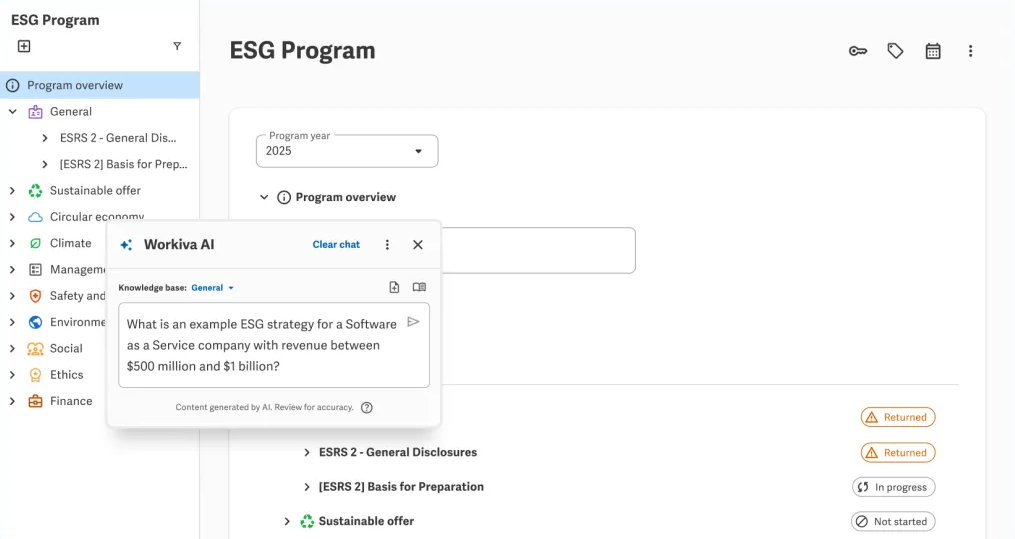
\includegraphics[width=5in]{frontmatter/assets/workiva.png}
%     \caption{Plataforma Workiva}
%     \label{fig:workiva}
% \end{figure}

\subsubsection{SAP Sustainability Control Tower}

O \textit{SAP Sustainability Control Tower} é uma solução SaaS\footnote{O SaaS, ou \textit{Software as a Service}, é um modelo de fornecimento de software baseado na nuvem (\textit{cloud}) em que os utilizadores acedem às aplicações através da Internet, em vez de as instalarem  localmente.} que permite às empresas registar, reportar e agir sobre métricas ESG com dados fiáveis e prontos para auditoria. Automatiza a integração de dados de múltiplas fontes, fornece cálculos avançados de emissões e incorpora \textit{insights} de sustentabilidade nos processos empresariais para uma gestão estratégica e transparente (\cite{SAP2025}).

\subsubsection{IBM Environmental Intelligence Suite}

O \textit{IBM Environmental Intelligence Suite} oferece APIs avançadas para integrar, analisar e visualizar dados ambientais, climáticos e de emissões de GEE\footnote{Emissões de gases com efeito de estufa (GEE).}. Ao usar \textit{machine learning} e \textit{AI-driven insights}, a plataforma permite extrair informações estratégicas, prever impactos e garantir conformidade com normas de sustentabilidade, adaptando-se às necessidades específicas de cada empresa (\cite{IBM2025}).

%-------------------------------------------------------------------------------
\subsection{Bibliotecas e Ferramentas de Desenvolvimento}
\label{subsec: BFD}

Esta subsecção aborda brevemente as ferramentas principais que serão usadas na solução desenvolvida.

\subsubsection{React.js}

O \textbf{React.js} é uma das bibliotecas\footnote{No contexto do \textit{React.js}, uma biblioteca é um conjunto de funcionalidades que pode utilizar para obter resultados que normalmente exigiriam mais código e trabalho da parte do utilizador.} \textit{JavaScript} de \textit{front-end} mais populares (\cite{Schwarzmuller2022}). O seu uso é focado na criação de interfaces de utilizador a partir de excertos de código individuais chamados \textbf{componentes} e das suas combinações em telas inteiras, páginas e aplicativos (\cite{React2025}).

\subsubsection{ApexCharts.js}

A \textbf{ApexCharts.js} é uma biblioteca de gráficos interativos \textit{open-source} em \textit{JavaScript}. Responsiva e de alto desempenho, permite criar visualizações dinâmicas com suporte a \textit{zoom}, \textit{scroll}, anotações e animações suaves. Oferece personalização avançada, incluindo gradientes, sombras e paletas de cores configuráveis, tornando-se uma solução eficiente para a visualização de dados na web (\cite{Apexcharts2025}).


 \vspace{20mm} 






\chapter{Análise do Problema}
\label{chap:AP}

Neste próximo Capítulo aborda-se a análise do problema em questão. Inicia-se com a descrição do domínio do problema através do glossário de termos usados, do modelo de domínio e do mapa de materialidade da Devscope de acordo com as métricas indicadas pela \gls{SASB} para o setor de \textit{software} e serviços IT. Por fim, serão elencados os requisitos funcionais e não funcionais do sistema.

\section{Contexto}
\label{sec:Context}

A fase de análise é uma das mais importantes no ciclo de vida do desenvolvimento de \textit{software}, pois é nela que ocorre a recolha dos requisitos, funcionalidades e necessidades do cliente, bem como das especificações do sistema. O objetivo final é definir de forma clara os recursos e funcionalidades que compõem a solução a ser desenvolvida.

Qualquer informação incorreta, ou não obtida, pode comprometer o desenvolvimento do produto, tanto em termos de qualidade como de cumprimento dos prazos.

A proposta de desenvolvimento de uma plataforma ESG surgiu da necessidade identificada pela Devscope em centralizar e otimizar o controlo de diversas métricas relacionadas com os pilares ambiental, social e de governança (ESG). Esta necessidade prende-se com a crescente importância de monitorizar e reportar práticas sustentáveis, promovendo uma gestão mais transparente, eficiente e alinhada com os objetivos de responsabilidade corporativa da empresa. Ao centralizar estes dados numa única plataforma, a Devscope pretende não só melhorar a sua capacidade de análise e tomada de decisões, como também reforçar o seu compromisso com a sustentabilidade e o impacto positivo na sociedade.

\section{Domínio do problema}
\label{sec:DP} 

A presente secção visa descrever o domínio do problema através de vários artefactos de complexidades diversas, nomeadamente conceitos e diagramas.

A Tabela \ref{tab:glossario_dominio} apresenta os conceitos de domínio do problema e que serão usados ao longo do desenvolvimento.

\begin{table}[H]
    \rowcolors{2}{purple!10}{white}
    \renewcommand{\arraystretch}{1.2}
    \setlength{\tabcolsep}{10pt}
    \centering
    \begin{tabular}{>{\bfseries}p{4cm} p{11cm}}
        \rowcolor{purple!40}
        \textbf{Conceito (EN)} & \textbf{Descrição} \\
        ESG & \textbf{ESG (Ambiente, Social e Governança)}: Conjunto de critérios que avaliam o desempenho ambiental, social e de governança de uma organização, com foco na sustentabilidade e responsabilidade corporativa. \\
        \textit{Dashboard} & \textbf{Painel}: Resumo gráfico de várias informações importantes, normalmente utilizado para dar uma visão geral de um negócio. \\
        \textit{Materiality Map} & \textbf{Mapa de Materialidade}: Ferramenta que destaca as métricas ESG mais relevantes para cada setor, segundo as normas da SASB. \\
        \textit{Metric} & \textbf{Métrica}: Unidade de medida usada para quantificar aspetos específicos do desempenho ESG, como emissões de carbono, diversidade na força de trabalho ou políticas anticorrupção. \\
        \textit{Dataset} & \textbf{Conjunto de Dados}: Coleção estruturada de dados ESG, normalmente em formato tabular, que contém informações como categorias, datas e valores associados. \\
        URL & \textbf{Localizador Uniforme de Recursos (URL)}: Endereço que identifica e localiza um recurso na internet, como páginas \textit{web}, APIs ou arquivos. \\
        API & \textbf{Interface de Programação de Aplicações (API)}: Conjunto de regras que permite a comunicação entre diferentes sistemas ou componentes de \textit{software}. Utilizada para integrar funcionalidades ou aceder a dados. \\
        KPI & \textbf{Indicador-Chave de Desempenho (KPI)}: Métrica usada para avaliar o sucesso de uma organização ou de uma atividade específica na conquista de objetivos estratégicos ou operacionais. \\
        SPA & \textbf{Aplicação de Página Única (SPA)}: Tipo de aplicação \textit{web} que carrega uma única página HTML e atualiza dinamicamente o conteúdo conforme o utilizador interage, sem recarregar completamente a página. \\
    \end{tabular}
    \caption{Glossário do domínio do problema}
    \label{tab:glossario_dominio}
\end{table}

A Figura \ref{fig:domain_model} ilustra uma visualização do modelo de domínio, traçando as relações entre os principais conceitos da solução pretendida. Cada uma das entidades principais foi especificada como uma raiz agregada, uma escolha motivada por preocupações de consistência transnacional, concorrência, escalabilidade e clareza semântica.

Um bom exemplo é a distinção entre \texttt{Empresa} e \texttt{Setor}. Enquanto o \texttt{Setor} caracteriza a empresa no contexto da indústria, também organiza o sistema agrupando as \texttt{Subáreas} e, por extensão, as \texttt{Métricas} relevantes para a avaliação ESG com base nas normas SASB. Ao representá-lo como um agregado autónomo, esta abordagem localiza a lógica subjacente, minimizando as redundâncias e promovendo a consistência.

\begin{figure}[H]
\centering
    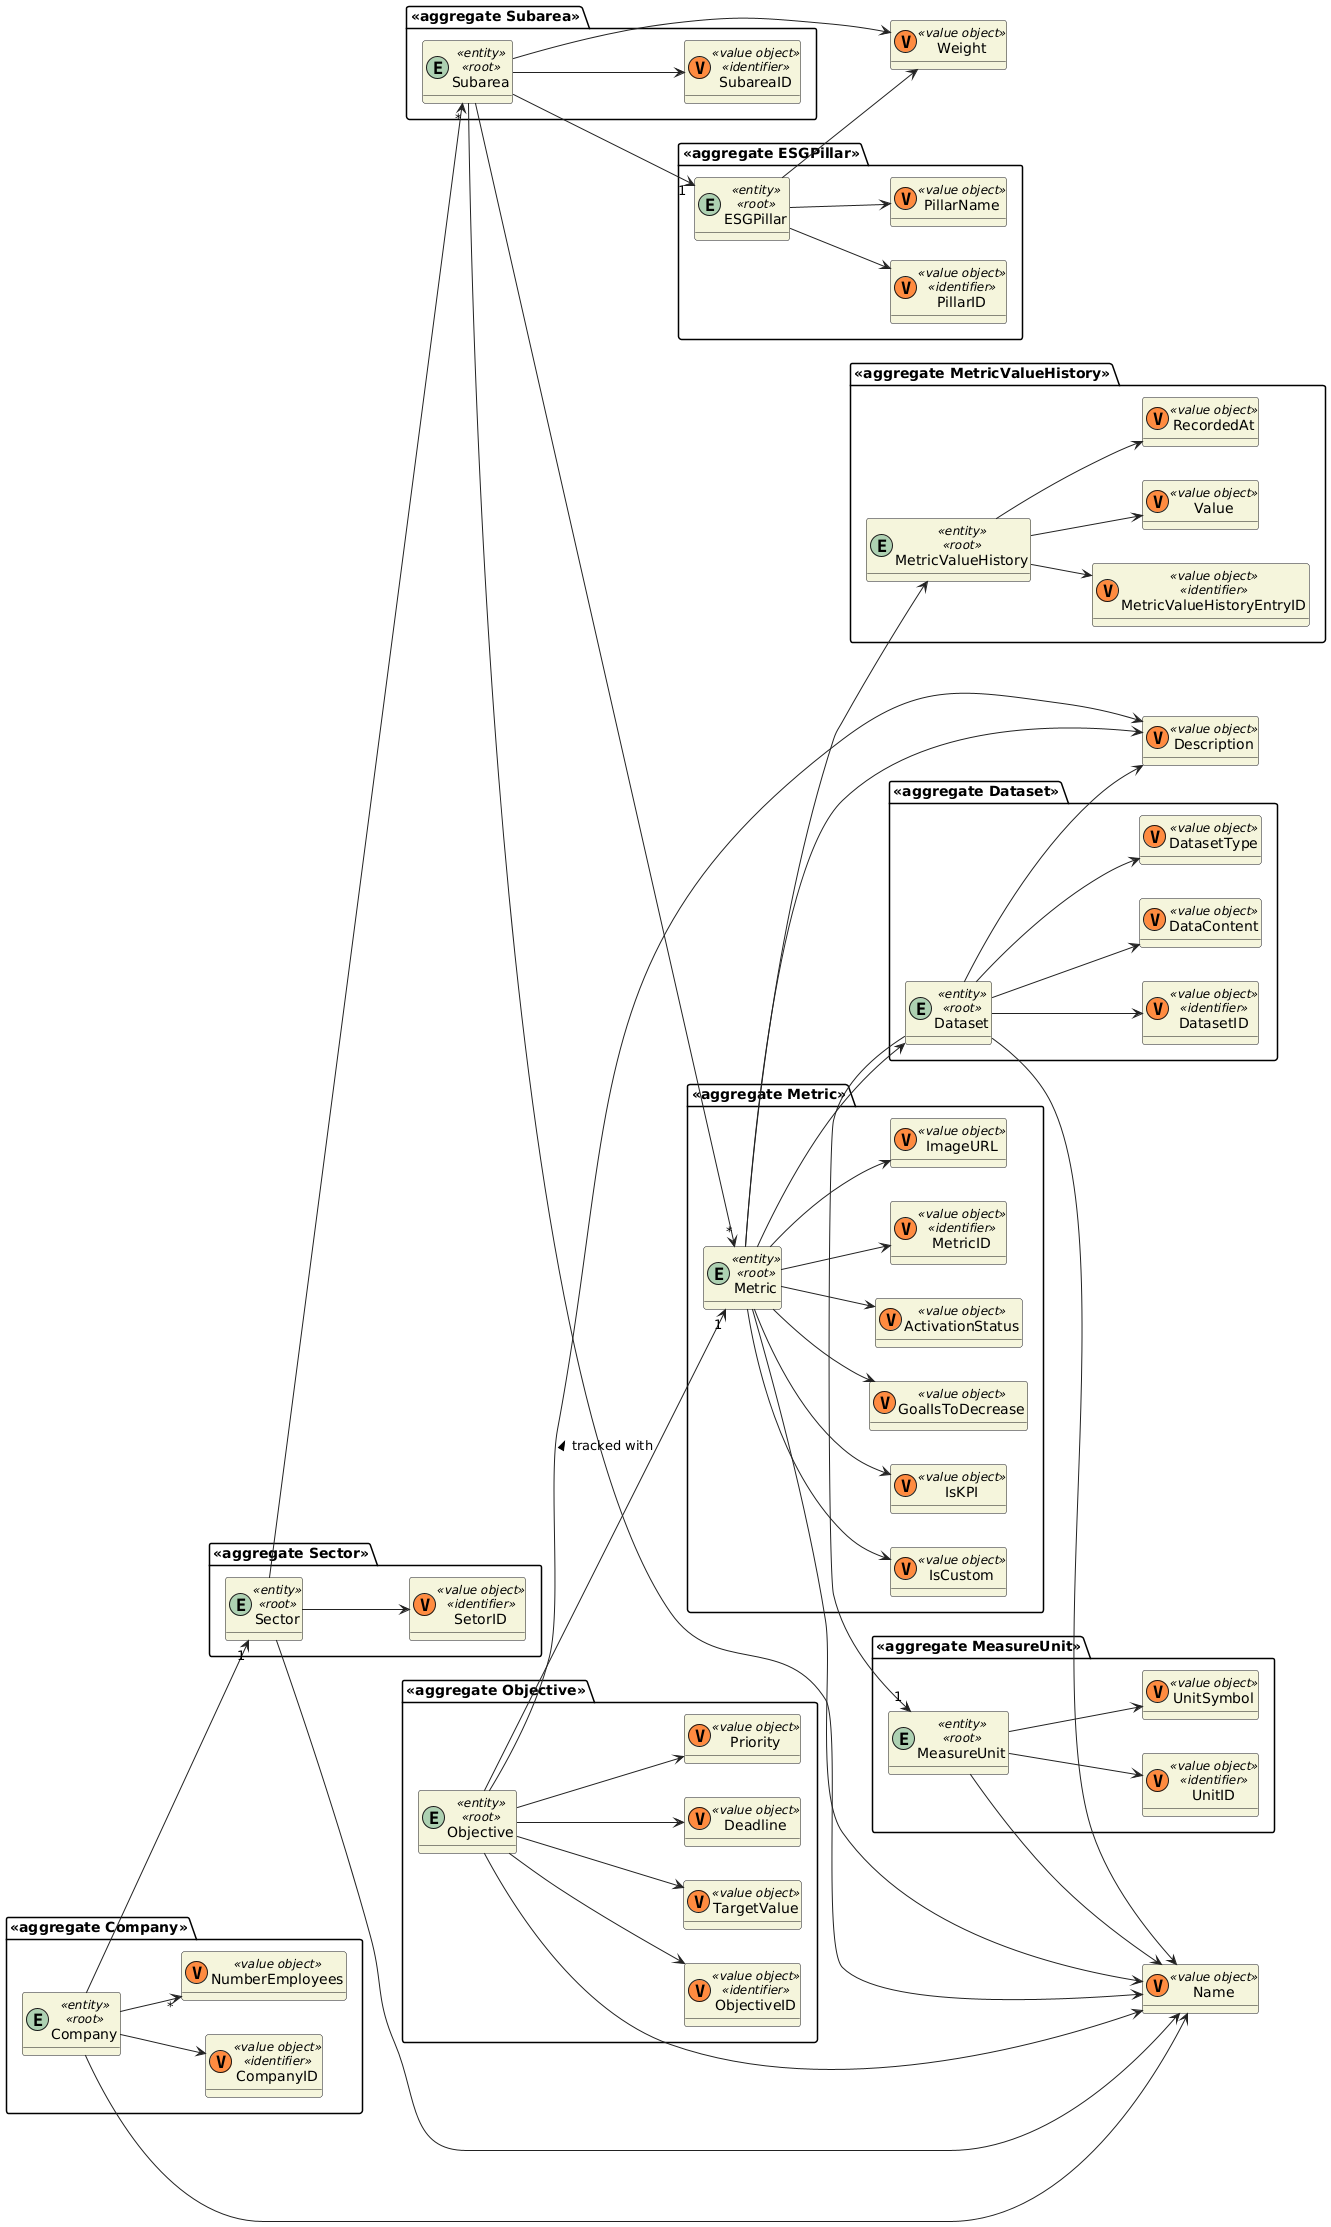
\includegraphics[width=\linewidth,keepaspectratio]{frontmatter/assets/diagrams/Domain Model/Domain_Model2.png}
    \caption{Modelo de Dominio (autoria própria)}
    \label{fig:domain_model}
\end{figure}


\subsection{Visão Geral da Aplicação}
\label{subsec:VGA} 

O \textit{dashboard} apresenta a pontuação ESG consolidada da empresa, oferecendo uma visão geral do seu desempenho em sustentabilidade. Além disso, destaca as métricas mais relevantes, assim como aquelas que apresentaram melhorias ou quedas em relação ao último registro.

Outra seção da plataforma disponibiliza uma visão detalhada de todas as métricas existentes: métricas customizáveis (criadas pelos próprios utilizadores) e métricas orientadas pelos padrões definidos pela \gls{SASB}.

Cada métrica possui atributos específicos, incluindo o pilar e subárea ESG a que pertence, o seu código identificador, os conjunto de dados que lhe estão associados, a unidade de medida associada aos mesmos e a classificação do seu progresso.

De acordo com a \gls{SASB}, adotado pela Devscope neste projeto, existem normas específicas para cada setor, como é o caso do setor de \textit{Software} e Serviços de TI, que determinam quais as métricas devem ser reportadas (\cite{SASBSector2025}). É com base nestas diretrizes que se constrói o Mapa de Materialidade, indicado na Figura \ref{fig:materiality_map}.

% - mapa de materialidade da DevScope (Software e IT sector - SASB)
\begin{figure}[H]
    \centering
    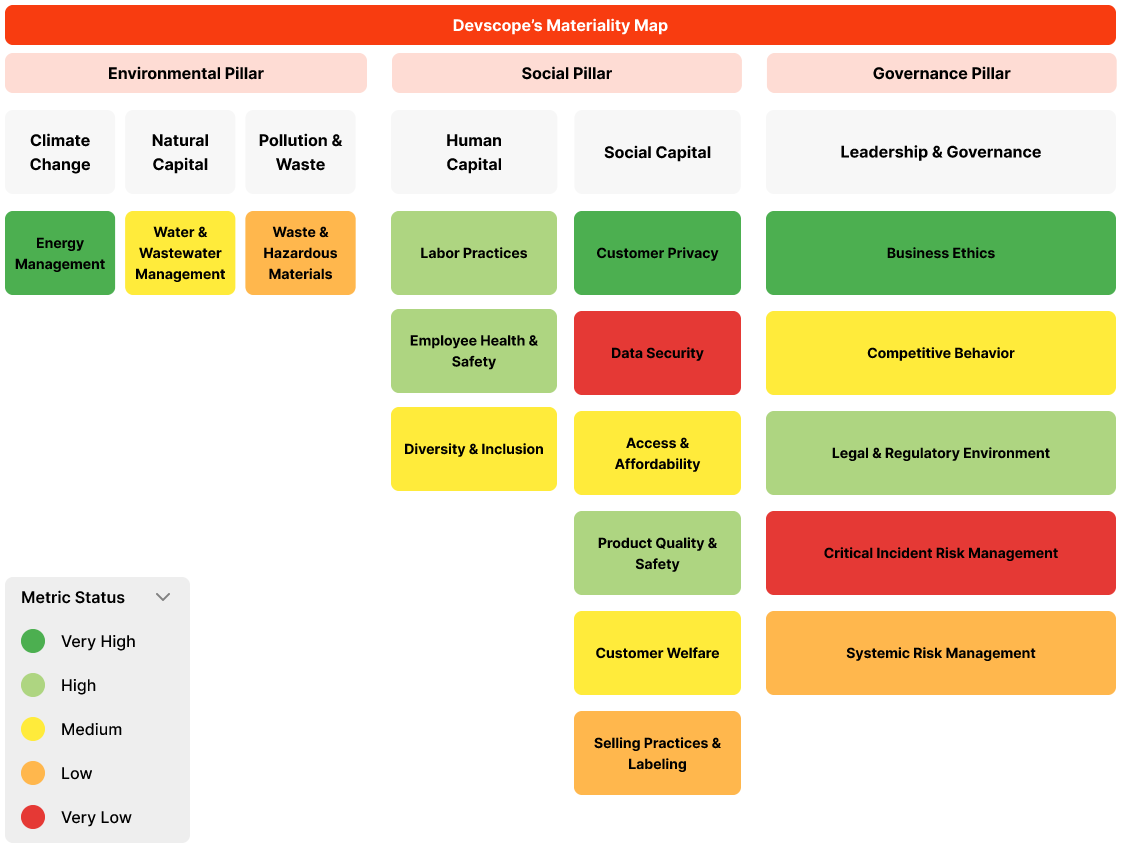
\includegraphics[width=5in]{frontmatter/assets/mapa-materialidade.png}
    \caption{Mapa de Materialidade segundo o setor SASB da Devscope (\textit{Software} e serviços IT) (autoria própria)}
    \label{fig:materiality_map}
\end{figure}

Neste mapa, um dos elementos centrais da plataforma, reflete as métricas ativas não só definidas pela \gls{SASB}, consoante o setor da empresa, bem como as métricas personalizadas. Este mapa organiza as métricas segundo os pilares ESG e respectivas subáreas, e atribui uma cor correspondente ao seu progresso, proporcionando uma visão estruturada das prioridades de sustentabilidade da organização.

Por fim, outra página da plataforma é dedicada à gestão de objetivos, permitindo acompanhar os objetivos definidos, as métricas a eles associadas, o progresso na sua concretização ao saber se se encontram dentro ou fora do plano estabelecido.

\section{Requisitos Funcionais e Não Funcionais}

Esta secção compila os requisitos obtidos com o cliente e categoriza-os entre funcionais e não funcionais.

\subsection{Requisitos Funcionais}
\label{subsec:FunReq}

Os requisitos funcionais correspondem a funcionalidades presentes no \textit{software} a ser desenvolvido, normalmente representadas por casos de uso e acompanhados por diagramas. Os requisitos funcionais deste projeto estão organizados na Tabela \ref{tab:use_cases}, onde cada requisito é considerado um caso de uso e identificado por um código alfa-numérico.

\begin{table}[H]
    \rowcolors{2}{orange!20}{white}
    \renewcommand{\arraystretch}{1.2}
    \setlength{\tabcolsep}{10pt}
    \centering
    \begin{tabular}{>{\bfseries}p{1.5cm} p{3.5cm} p{8cm}}
        \rowcolor{orange!50}
        Código & \textbf{Descrição Curta} & \textbf{Descrição} \\
        UC-01 & Visualização de KPI's & Como utilizador da plataforma, quero visualizar rapidamente os principais KPIs ambientais, sociais e de governação, para poder avaliar o desempenho da organização. \\
        UC-02 & Filtragem de Métricas & Como utilizador da plataforma, quero poder filtrar os dados por pilar, de modo a facilitar a navegação. \\
        UC-03 & Mapa de Materialidade & Como utilizador da plataforma, quero visualizar a matriz de materialidade dividida por categorias ESG com um sistema de cores intuitivo, para identificar rapidamente os temas mais críticos e, ao clicar em cada indicador, aceder a detalhes explicativos que me ajudem a compreender o seu progresso e evolução. \\
        UC-04 & Pontuação ESG & Como utilizador da plataforma, quero aceder a uma pontuação ESG agregada, para ter uma visão geral do desempenho da empresa em responsabilidade social, ambiental e de governança. \\
        UC-05 & Detalhes de Métricas & Como utilizador da plataforma, quero clicar numa métrica e ver mais detalhes, para compreender a progressão de cada indicador. \\
        UC-06 & Métricas Customizáveis & Como utilizador da plataforma, quero poder criar métricas ESG específicas à realidade da empresa e definir a sua fonte de dados, para garantir que o painel reflete os indicadores mais relevantes para a nossa estratégia. \\
        UC-07 & Importação de Dados & Como utilizador da plataforma, quero poder importar dados para associar às métricas. \\      
    \end{tabular}
    \caption{Lista de Casos de Uso}
    \label{tab:use_cases}
\end{table}

A Figura \ref{fig:scenario_view} é um diagrama que compila os caso de usos principais do projeto, que serão apresentados de forma detalhada.

\begin{figure}[H]
    \centering
    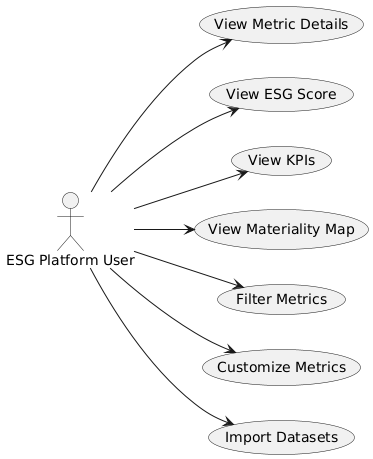
\includegraphics[height=4in,keepaspectratio]{frontmatter/assets/diagrams/Scenario View/Scenario_View.png}
    \caption{Vista de Cenários (autoria própria)}
    \label{fig:scenario_view}
\end{figure}

\subsubsection{UC-01 | Visualização de KPI's}

\textbf{Objetivo:} Permitir ao utilizador consultar rapidamente os principais \textit{\gls{KPI}} ESG da organização. \\
\textbf{Ator Principal:} Utilizador da plataforma \\
\textbf{Descrição Geral:} Este caso de uso disponibiliza uma visão geral de métricas dos três pilares (Ambiental, Social e de Governação). A interface mostra indicadores como emissões de CO$_2$, diversidade na força de trabalho, entre outros. \\
\textbf{Fluxo Principal:}
\begin{enumerate}
    \item O utilizador acede ao painel principal da plataforma.
    \item A aplicação apresenta os KPIs.
    \item O utilizador pode visualizar valores atuais e tendências.
\end{enumerate}
\textbf{Resultado Esperado:} O utilizador obtém uma perceção imediata do desempenho ESG da empresa.

\subsubsection{UC-02 | Filtragem de Métricas}

\textbf{Objetivo:} Permitir ao utilizador filtrar os dados por pilar ESG (\textit{Environmental}, \textit{Social} ou \textit{Governance}).\\
\textbf{Ator Principal:} Utilizador da plataforma\\
\textbf{Descrição Geral:} Este caso de uso oferece um mecanismo de filtragem que facilita a navegação por métricas, de acordo com o pilar de interesse.\\
\textbf{Fluxo Principal:}
\begin{enumerate}
    \item O utilizador seleciona o pilar desejado através de controlos de filtragem.
    \item A plataforma atualiza os dados apresentados para refletir apenas as métricas relevantes.
\end{enumerate}
\textbf{Resultado Esperado:} O utilizador consegue concentrar-se nos dados ESG mais relevantes ao seu objetivo de análise.

\subsubsection{UC-03 | Mapa de Materialidade}

\textbf{Objetivo:} Exibir uma matriz de materialidade com base no setor da empresa, permitindo a priorização de temas ESG.\\
\textbf{Ator Principal:} Utilizador da plataforma\\
\textbf{Descrição Geral:} A matriz destaca os temas ESG mais críticos segundo o modelo SASB, com categorização por pilar e subárea, e códigos de cor para facilitar a interpretação.\\
\textbf{Fluxo Principal:}
\begin{enumerate}
    \item O utilizador acede à secção de materialidade.
    \item É apresentada a matriz correspondente ao setor da empresa.
    \item O utilizador pode clicar em indicadores para visualizar descrições detalhadas.
\end{enumerate}
\textbf{Resultado Esperado:} Facilita a identificação de prioridades estratégicas ESG para o setor em análise.

\subsubsection{UC-04 | Pontuação ESG}

\textbf{Objetivo:} Fornecer uma pontuação ESG agregada para a empresa.\\
\textbf{Ator Principal:} Utilizador da plataforma\\
\textbf{Descrição Geral:} A aplicação calcula e exibe uma pontuação ESG com base nas métricas existentes e ativas, representada por cores e uma escalas numéricas.\\
\textbf{Fluxo Principal:}
\begin{enumerate}
    \item O utilizador acede ao \textit{dashboard} principal.
    \item A plataforma mostra a pontuação global da empresa.
    \item Podem existir dicas ou justificações para a pontuação.
\end{enumerate}
\textbf{Resultado Esperado:} Oferece uma visão sintética do desempenho ESG.

\subsubsection{UC-05 | Detalhes de Métricas}

\textbf{Objetivo:} Permitir a exploração detalhada de cada métrica ESG.\\
\textbf{Ator Principal:} Utilizador da plataforma\\
\textbf{Descrição Geral:} O utilizador pode selecionar uma métrica para visualizar dados históricos, a classificação do seu progresso, o conjunto de dados de origem e o pilar e subárea a que pertence.\\
\textbf{Fluxo Principal:}
\begin{enumerate}
    \item O utilizador clica numa métrica apresentada em \textit{dashboards} ou gráficos.
    \item A aplicação apresenta uma vista detalhada com gráficos temporais, dados e metadados.
\end{enumerate}
\textbf{Resultado Esperado:} Maior compreensão do desempenho de cada indicador específico.

\subsubsection{UC-06 | Métricas Customizáveis}

\textbf{Objetivo:} Permitir ao utilizador definir novas métricas ESG alinhadas com a realidade da empresa.\\
\textbf{Ator Principal:} Utilizador da plataforma\\
\textbf{Descrição Geral:} Funcionalidade que permite criar métricas personalizadas, associando-as a fontes de dados e subáreas ESG específicas.\\
\textbf{Fluxo Principal:}
\begin{enumerate}
    \item O utilizador acede à área de configuração de métricas.
    \item Define os dados pedidos.
    \item A métrica é validada e integrada nos \textit{dashboards}.
\end{enumerate}
\textbf{Resultado Esperado:} Flexibilidade para adaptar o sistema ESG a diferentes contextos empresariais.

\subsubsection{UC-07 | Importação de Dados}

\textbf{Objetivo:} Permitir ao utilizador importar conjuntos de dados em formato CSV para análise ESG.\\
\textbf{Ator Principal:} Utilizador da plataforma\\
\textbf{Descrição Geral:} O utilizador pode carregar ficheiros de dados externos, que serão associados a métricas e utilizados em gráficos e cálculos.\\
\textbf{Fluxo Principal:}
\begin{enumerate}
    \item O utilizador escolhe o ficheiro CSV a importar.
    \item O sistema valida o conteúdo.
    \item As informações passam a estar disponíveis para visualização e análise.
\end{enumerate}
\textbf{Resultado Esperado:} Capacidade de integração de dados externos no ecossistema ESG da aplicação.


\subsection{Requisitos Não Funcionais}

Requisitos não funcionais correspondem a todas as propriedades do sistema que não se referem diretamente a funcionalidades específicas, mas sim a qualidades e restrições sobre como o sistema se deve comportar. Incluem aspetos como desempenho, usabilidade, confiabilidade, manutenibilidade e outros fatores de qualidade da aplicação.

Uma forma amplamente utilizada de categorizar estes requisitos é através do modelo \textbf{FURPS+}, detalhado na Tabela \ref{tab:furps}, que cataloga os requisitos não funcionais em cinco categorias principais, com um grupo adicional representado pelo símbolo \texttt{+}.

\begin{table}[H]
    \rowcolors{2}{blue!30}{white}
    \renewcommand{\arraystretch}{1.2}
    \setlength{\tabcolsep}{10pt}
    \centering
    \begin{tabular}{>{\bfseries}p{1cm} >{\bfseries}p{2.5cm} p{10cm}}
        \rowcolor{blue!50}
        Letra & Categoria & Descrição \\
        F & \textit{Functionality} & Funcionalidades esperadas, segurança, interoperabilidade e adequação funcional \\
        U & \textit{Usability} & Facilidade de uso, aparência, acessibilidade, e interação com o utilizador \\
        R & \textit{Reliability} & Confiabilidade, tolerância a falhas, disponibilidade, e recuperação \\
        P & \textit{Performance} & Tempo de resposta, eficiência de recursos e escalabilidade \\
        S & \textit{Supportability} & Facilidade de manutenção, extensibilidade, modularidade, e testabilidade \\
        + & \textit{Others} & Restrições de design, implementação, normas, tecnologias ou frameworks \\
    \end{tabular}
    \caption{Categorias FURPS+}
    \label{tab:furps}
\end{table}

Os tópicos seguintes categorizam os requisitos não funcionais obtidos consoante o modelo FURPS+.

\subsection{\textit{Usabilidade (U)}}
\begin{itemize}
    \item \textit{Feedback} imediato ao utilizador através de alertas indicando sucesso ou erro das ações realizadas.
    \item Interface do utilizador em inglês para facilitar o acesso global.
\end{itemize}

\subsection{\textit{Confiabilidade (R)}}
\begin{itemize}
    \item O sistema deve apresentar mensagens de erro claras e específicas, indicando a origem do problema, em pelo menos 95\% dos casos de falha.
\end{itemize}

\subsection{\textit{Performance (P)}}
\begin{itemize}
    \item As interações principais devem ser eficientes e não exceder 30 segundos por operação.
    \item O tempo total para utilizar a prova de conceito (incluindo \textit{seeding} de dados e carregamento da interface) não deve ultrapassar 3 minutos.
\end{itemize}

\subsection{\textit{Suportabilidade (S)}}
\begin{itemize}
    \item Conformidade com o padrão \gls{SASB} para estruturação das métricas \gls{ESG}.
    \item A arquitetura do sistema deve permitir a adição de novas funcionalidades com impacto mínimo na base de código existente e sem degradação da usabilidade.
\end{itemize}

\subsection{+ (Outros)}
\begin{itemize}
    \item Seguir boas práticas de programação e arquitetura coesa.
    \item Utilizar fonte de dados simulada através de scripts de seeding.
    \item Comunicação entre os diferentes módulos da aplicação através de REST APIs utilizando HTTP/S para garantir interoperabilidade e segurança.
    \item Devem ser implementados testes unitários e de integração cobrindo, no mínimo, 80\% das funcionalidades críticas do sistema.
    \item Código modular e bem estruturado, seguindo princípios de separação de responsabilidades.
    \item Arquitetura baseada em boas práticas, como \textit{Clean Architecture} e uso de camadas (\textit{Controller, Service, Repository}).
\end{itemize}

%-------------------------------------------------------------------------------

\chapter{Desenho da solução}
\label{chap:DS}

Este capítulo aborda a fase de \textit{design} no processo de desenvolvimento de \textit{software}, onde, após a recolha de requisitos e análise das funcionalidades, são delineados os elementos do sistema através de diagramas que refletem a arquitetura e os modelos escolhidos, tendo em conta os requisitos e restrições definidos. Conforme descrito em \cite{tsui2022essentials}, o \textit{design} é dividido em duas etapas principais:

\begin{itemize}
    \item \textbf{Design arquitetural} — uma visão macro e de alto Nível do sistema, onde são identificados os principais componentes, as suas propriedades externas e as relações entre eles. Esta fase é orientada pelos requisitos funcionais e não funcionais, bem como por considerações técnicas;
    \item \textbf{Design detalhado} — uma decomposição mais pormenorizada dos componentes, que detalha como cada módulo cumpre os requisitos funcionais definidos. Esta fase representa uma visão micro do sistema, guiada pela arquitetura estabelecida e pelos requisitos funcionais.
\end{itemize}


\section{Arquitetura do Sistema} 

\subsection{\textit{Clean Architecture}}

A \textit{Clean Architecture} é um modelo arquitetural de \textit{software} que privilegia a manutenibilidade e a escalabilidade do sistema, ao restringir as dependências entre os componentes de diferentes camadas. Neste modelo, diz-se que um componente A depende de um componente B se A conhece diretamente o nome de B, por exemplo, se o importa ou referencia. O objetivo da \textit{Clean Architecture} é limitar estas dependências para que alterações em uma parte do sistema não causem efeitos colaterais noutras. Para isso, aplica-se o princípio da inversão de dependências: o componente A define uma interface, e o componente B implementa essa interface. Mesmo que A chame B em tempo de execução, B é quem depende de A, pois precisa de conhecer e implementar a interface definida por A (\cite{Lano2023}).

Segundo \cite{Lano2023}, este princípio está na base da chamada regra de dependência, que afirma que componentes dependentes de plataformas externas (como bases de dados, \textit{frameworks} ou interfaces gráficas) podem depender da lógica de negócio, mas nunca o contrário. Assim, a lógica central do sistema permanece isolada e protegida de alterações tecnológicas periféricas, garantindo maior estabilidade e facilidade de evolução ao longo do tempo.

A Figura \ref{fig:cleanArchitecture} ilustra o modelo \textit{Clean Architecture} e as suas camadas concêntricas.

\begin{figure}[H]
    \centering
    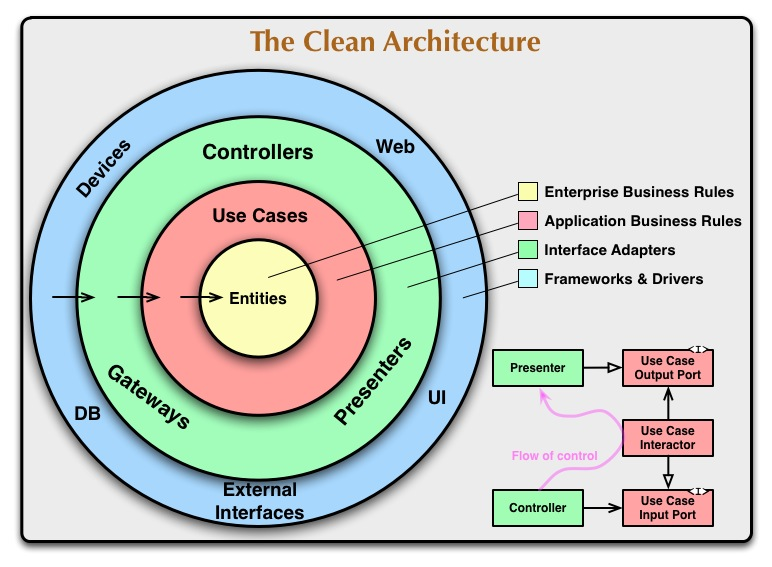
\includegraphics[width=5.5in,keepaspectratio]{frontmatter/assets/models/CleanArchitecture.jpg}
    \caption{Modelo Arquitural \textit{Clean Architecture} (\cite{Martin2012})}
    \label{fig:cleanArchitecture}
\end{figure}

Embora o projeto se inspire nos princípios da \textit{Clean Architecture}, nomeadamente a separação clara entre as camadas de apresentação, lógica de negócio e acesso a dados, não foi realizada uma implementação rigorosa deste modelo (por exemplo, com injeção de dependências ou uso sistemático de interfaces). Esta decisão deve-se ao âmbito do projeto e à sua natureza prática, que não exigem este Nível de abstração.

Em alternativa à implementação deste modelo, foram aplicados os modelos C4 (Figura \ref{subsec:modelC4}) e “4+1” (Figura \ref{subsec:model4plus1}) para representar graficamente a arquitetura da solução, proporcionando uma visão clara e compreensível da estrutura do sistema e das suas interações.


\subsection{Modelo C4}
\label{subsec:modelC4}

O modelo C4 descreve a arquitetura de um \textit{software} em quatro níveis de detalhe (\textit{Context, containers, components} e \textit{code}). De modo a criar os diferentes diagramas é necessario diferentes graus de abstração (\cite{Brown2018}):

\begin{itemize}
    \item \textbf{(Nível 1) \textit{System context diagram} -} Dá uma vista geral do contexto em que o sistema se insere, isto é, quem usa o \textit{software} criado e como é que outros sistemas inseridos no mesmo contexto comunicam com ele. 
    \item \textbf{(Nível 2) \textit{Container diagram} -} Detalha o sistema a um nível macro, decompondo-o em "\textit{containers}", tais como aplicações (monolíticas ou microsserviços), armazenamentos de dados, entre outros.
    \item \textbf{(Nível 3) \textit{Component diagram} -} Decompõe um \textit{container} em elementos que constituem abstrações reais no código a ser produzido.
    \item \textbf{(Nível 4) \textit{Code} -} Nível de detalhe final, define a implementação de um componente.
\end{itemize}

A Figura \ref{fig:c4model} hierarquiza a granularidade pretendida no detalhe das diferentes visões do sistema numa representação com o modelo C4.

\begin{figure}[H]
    \centering
    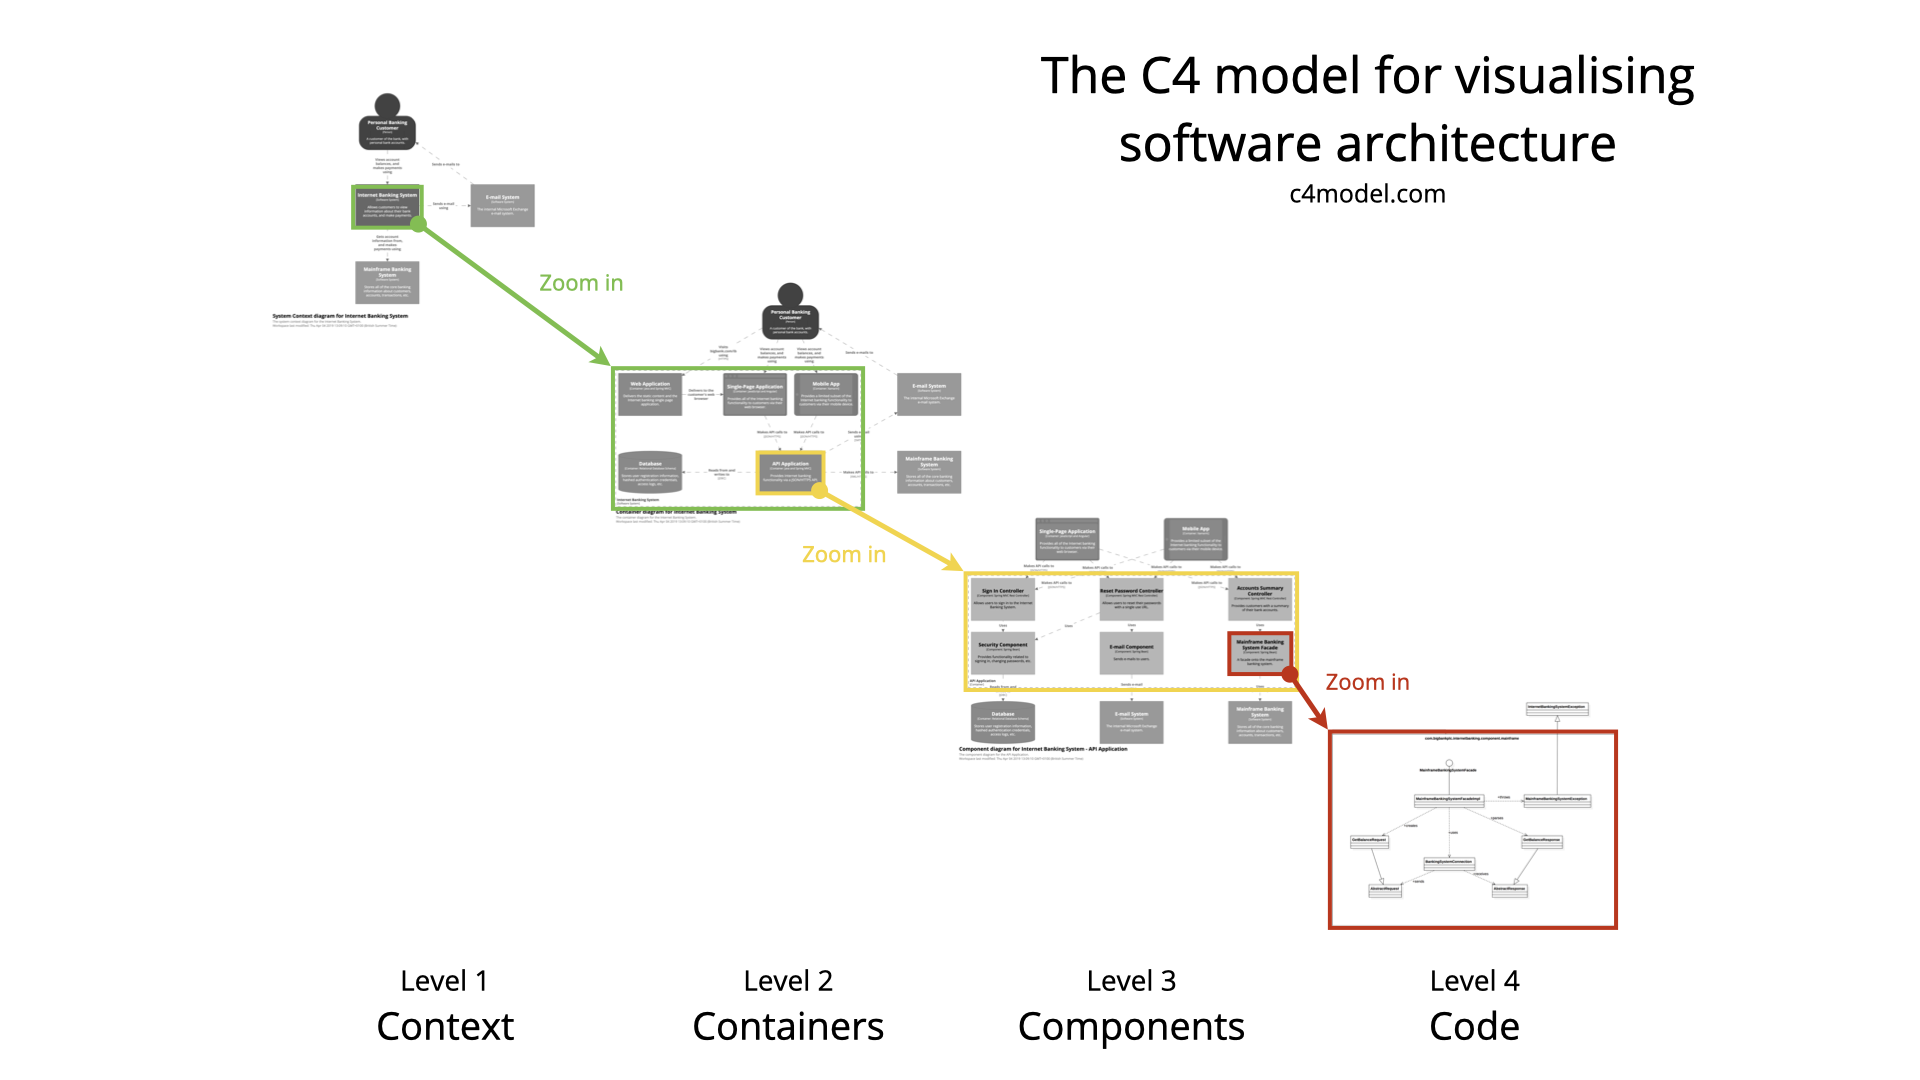
\includegraphics[width=6.5in,keepaspectratio]{frontmatter/assets/models/c4-overview.png}
    \caption{Modelo Arquitural C4 (\cite{C4Model})}
    \label{fig:c4model}
\end{figure}

A granularidade do Nível 4 revela-se excessiva e retira o foco aos diagramas que melhor ilustram a arquitetura do sistema, portanto, nao será abordado neste relatório.

\subsection{Modelo de Vistas 4+1}
\label{subsec:model4plus1}

Segundo \cite{Kruchten1995}, o modelo arquitetural "4+1" descreve a arquitetura de um sistema de \textit{software} a partir de cinco perspetivas complementares, cada uma focada em diferentes preocupações e públicos-alvo:

\begin{itemize}
\item \textbf{Vista Lógica -} Foca-se na funcionalidade do sistema, pois representa a estrutura dos principais componentes do domínio.

\item \textbf{Vista de Processos -} Descreve os aspectos dinâmicos do sistema, como a comunicação entre processos concorrentes e a forma como as tarefas são sincronizadas e distribuídas.

\item \textbf{Vista Física -} Mapeia os componentes de \textit{software} para os recursos de \textit{hardware} e ilustra como o sistema está distribuídoo.

\item \textbf{Vista de Implementação/Desenvolvimento -} Mostra a estrutura estática do código, organização em módulos/pacotes e o ambiente de desenvolvimento.

\item \textbf{Vista de Cenários -} Representa os principais casos de uso ou fluxos de interação do sistema.
\end{itemize}

A Figura \ref{fig:41viewmodel} ilustra as diferentes vistas, o respetivo público-alvo para cada uma, e as suas interações.

\begin{figure}[H]
    \centering
    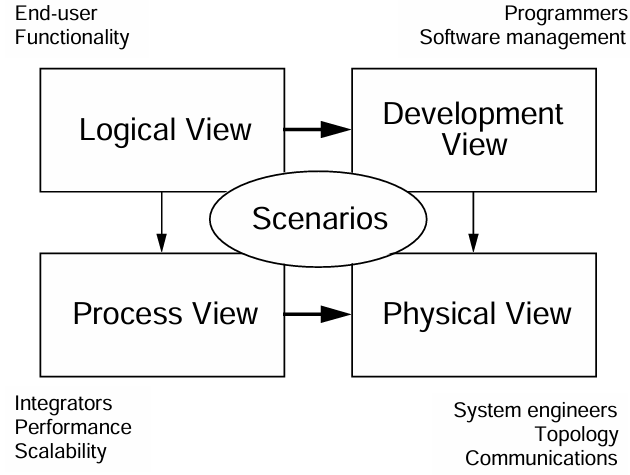
\includegraphics[width=3in,keepaspectratio]{frontmatter/assets/models/4+1views.png}
    \caption{Modelo de Vistas "4+1" (\cite{Kruchten1995})}
    \label{fig:41viewmodel}
\end{figure}

\subsection{Vista de Processos}
\label{subsec:process_view}

Alguns casos de uso partilham entre si a mesma estrutura de interação representada nos diagramas da vista de processos. Exemplos disso são os casos de uso UC-01, UC-02, UC-03, UC-04 e UC-05, que seguem a sequência ilustrada na Figura \ref{fig:UC12345-lvl1}, variando apenas no conceito de negócio específico que cada um aborda.

\begin{figure}[h]
\centering
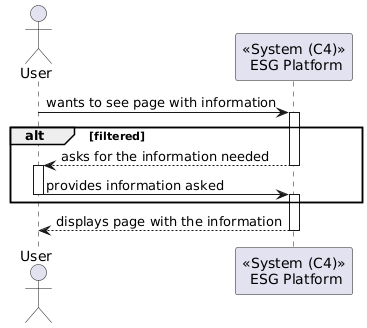
\includegraphics[width=3.5in]{frontmatter/assets/diagrams/Process Views/UC12345-lvl1.png}
\caption{Vista de processos dos casos de uso de consulta/visualização e filtragem (Nível 1) (autoria própria)}
\label{fig:UC12345-lvl1}
\end{figure}

De igual forma, os respetivos diagramas de Nível 2 também partilham uma estrutura comum, diferenciando-se apenas na lógica de negócio subjacente. Esta semelhança é evidenciada na Figura \ref{fig:UC12345-lvl2}, que exemplifica uma dessas variações mantendo a arquitetura processual de base.

\begin{figure}[H]
\centering
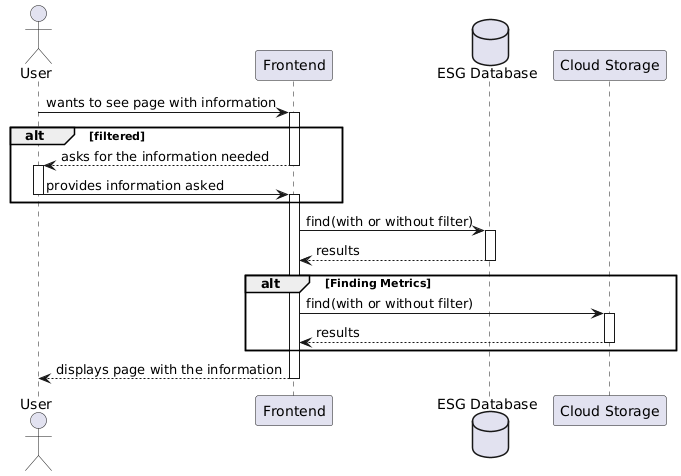
\includegraphics[width=5in]{frontmatter/assets/diagrams/Process Views/UC12345-lvl2.png}
\caption{Vista de processos dos casos de uso de consulta/visualização e filtragem (Nível 2) (autoria própria)}
\label{fig:UC12345-lvl2}
\end{figure}

É no Nível 3 que se tornam evidentes as diferenças nos fluxos de interação, consoante os requisitos de cada funcionalidade. Como ilustrado na Figura \ref{fig:UC134-lvl3}, os casos de uso UC-01, UC-03 e UC-04 envolvem apenas o acesso à base de dados.

\begin{figure}[H]
\centering
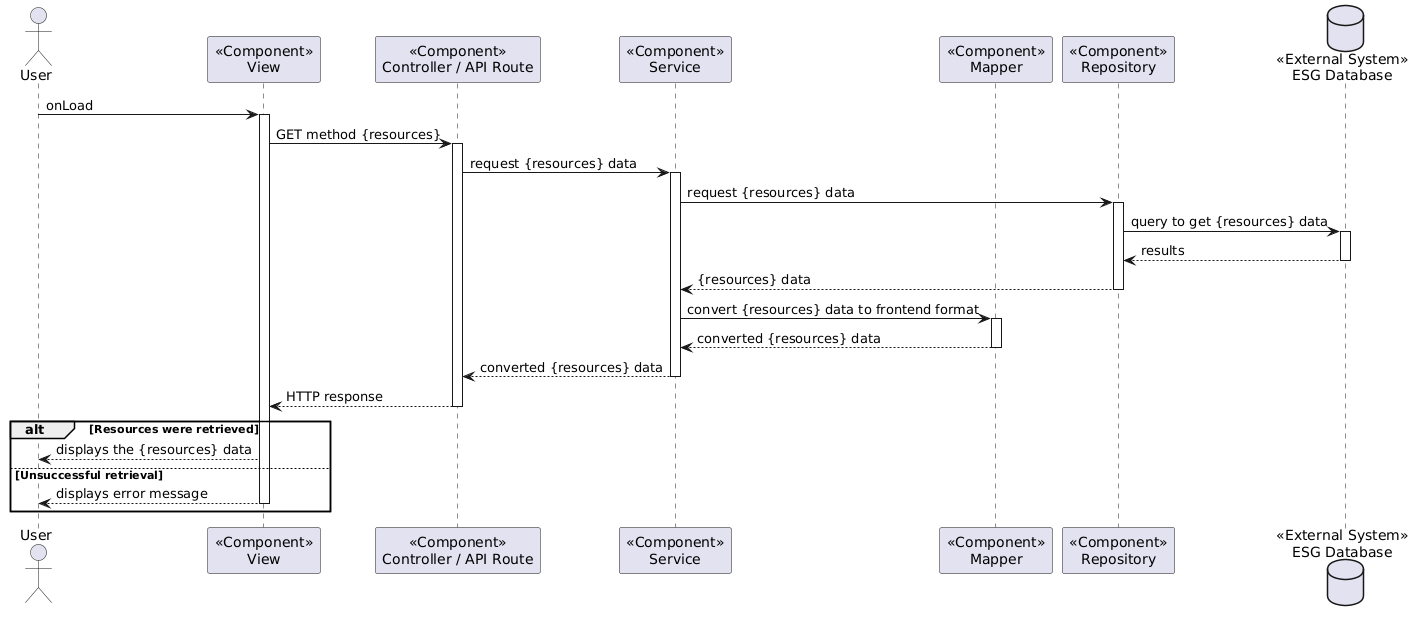
\includegraphics[width=\linewidth]{frontmatter/assets/diagrams/Process Views/LVL3/uc134-lvl3.png}
\caption{Vista de processos dos casos de uso de consulta (Nível 3) (autoria própria)}
\label{fig:UC134-lvl3}
\end{figure}

Já o caso UC-05 (Figura \ref{fig:UC5-lvl3}) inclui também comunicação com o serviço de armazenamento na nuvem.

\begin{figure}[H]
\centering
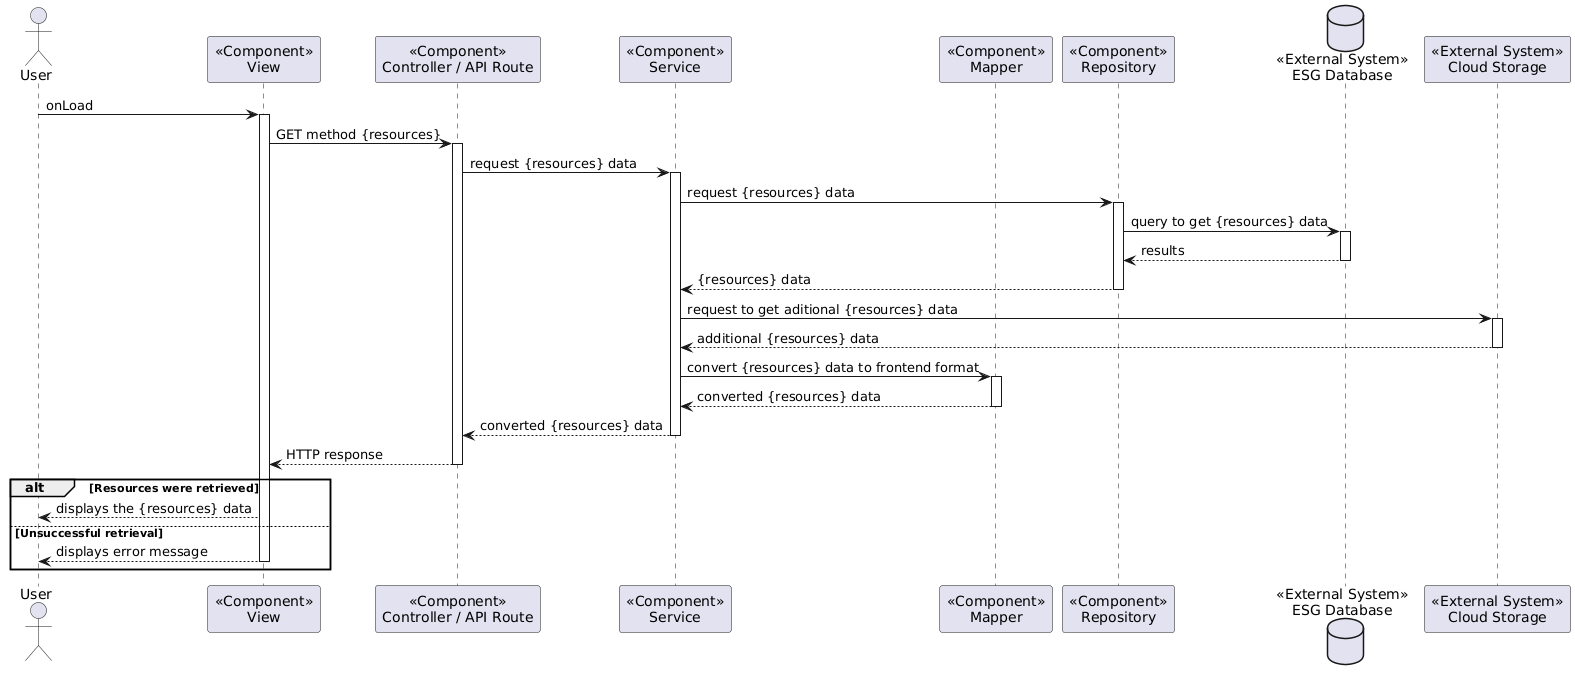
\includegraphics[width=\linewidth]{frontmatter/assets/diagrams/Process Views/LVL3/uc-05-lvl3.png}
\caption{Vista de processo do caso de uso de consulta com acesso ao armazenamento na nuvem (Nível 3) (autoria própria)}
\label{fig:UC5-lvl3}
\end{figure}

A UC-02 (Figura \ref{fig:UC2-lvl3}) distingue-se ainda por incluir uma etapa de filtragem adicional antes da obtenção dos dados.

\begin{figure}[H]
\centering
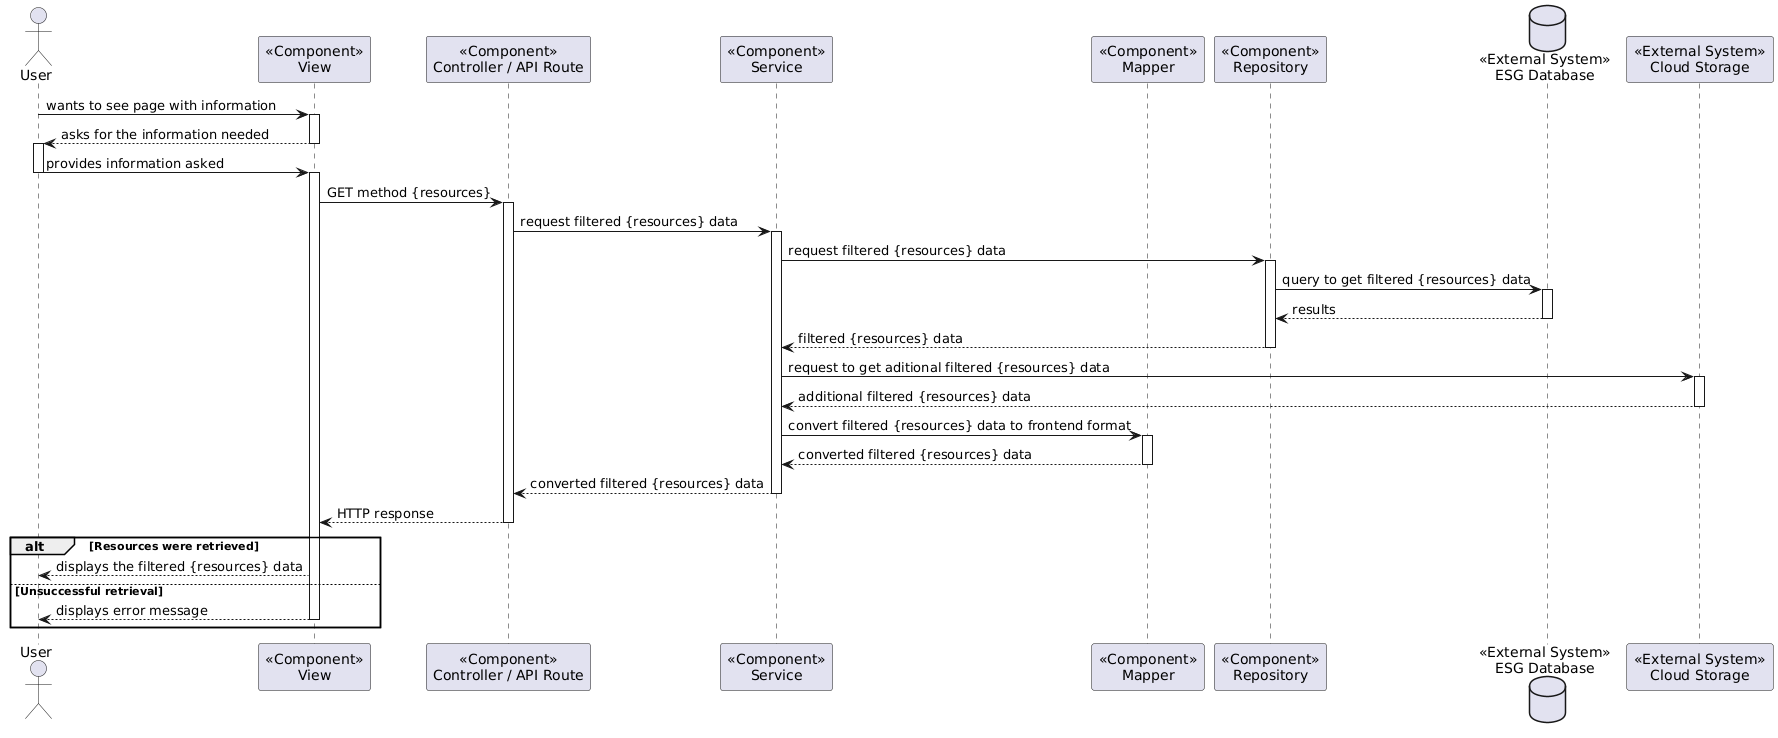
\includegraphics[width=\linewidth]{frontmatter/assets/diagrams/Process Views/LVL3/uc-02-lvl3.png}
\caption{Vista de processo do caso de uso de filtragem (Nível 3) (autoria própria)}
\label{fig:UC2-lvl3}
\end{figure}

Da mesma forma, no Nível 1, ambas os casos de uso UC-06 e UC-07 são bastante semelhantes, mudando apenas a lógica do negócio, como é ilustrado na Figura \ref{fig:UC67-lvl1}.

\begin{figure}[H]
\centering
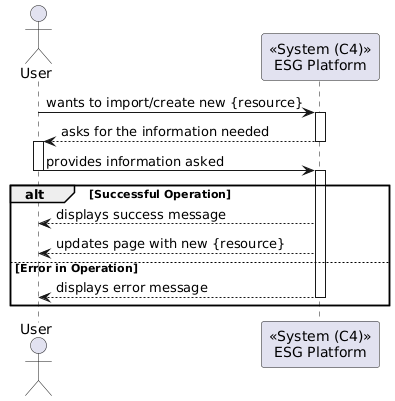
\includegraphics[width=3in]{frontmatter/assets/diagrams/Process Views/UC67-lvl1.png}
\caption{Vista de processo dos casos de uso de criação e importação (Nível 1) (autoria própria)}
\label{fig:UC67-lvl1}
\end{figure}

A mesma tendência continua no nível seguinte, como é representado pela Figura \ref{fig:UC67-lvl2}.

\begin{figure}[H]
\centering
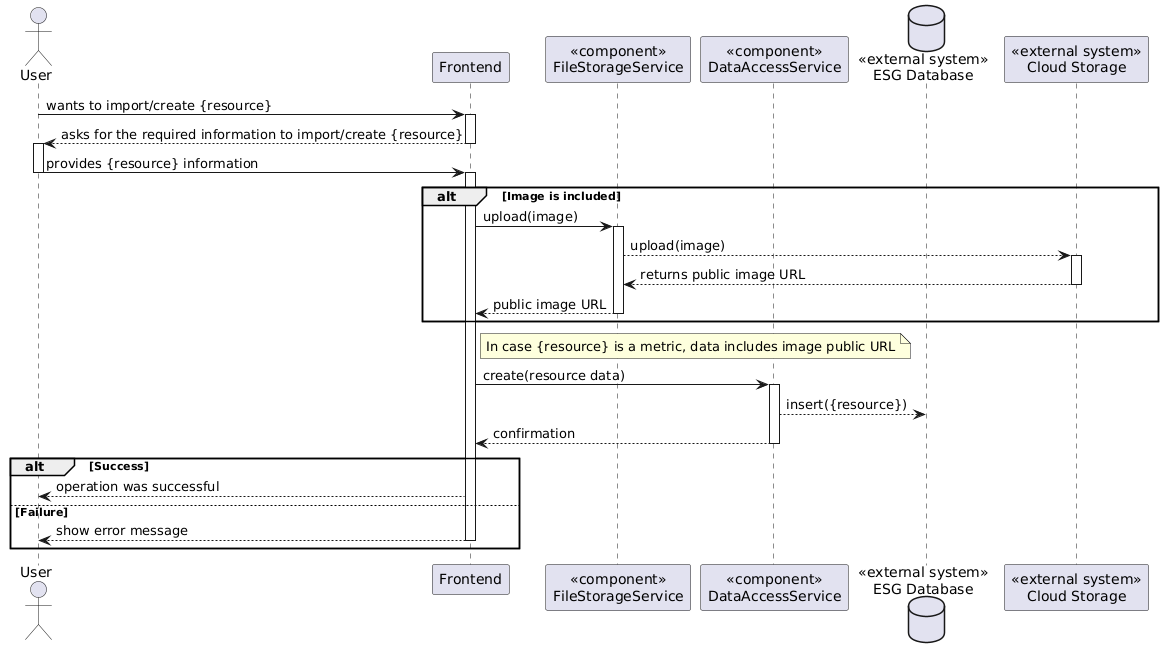
\includegraphics[width=\linewidth]{frontmatter/assets/diagrams/Process Views/UC67-lvl2.png}
\caption{Vista de processo dos casos de uso de criação e importação (Nível 2) (autoria própria)}
\label{fig:UC67-lvl2}
\end{figure}

A diferença no caso de uso UC-06 é realçada pelo diagrama de granularidade de Nível 3, como se pode ver na Figura \ref{fig:UC6-lvl3}.

\begin{figure}[H]
\centering
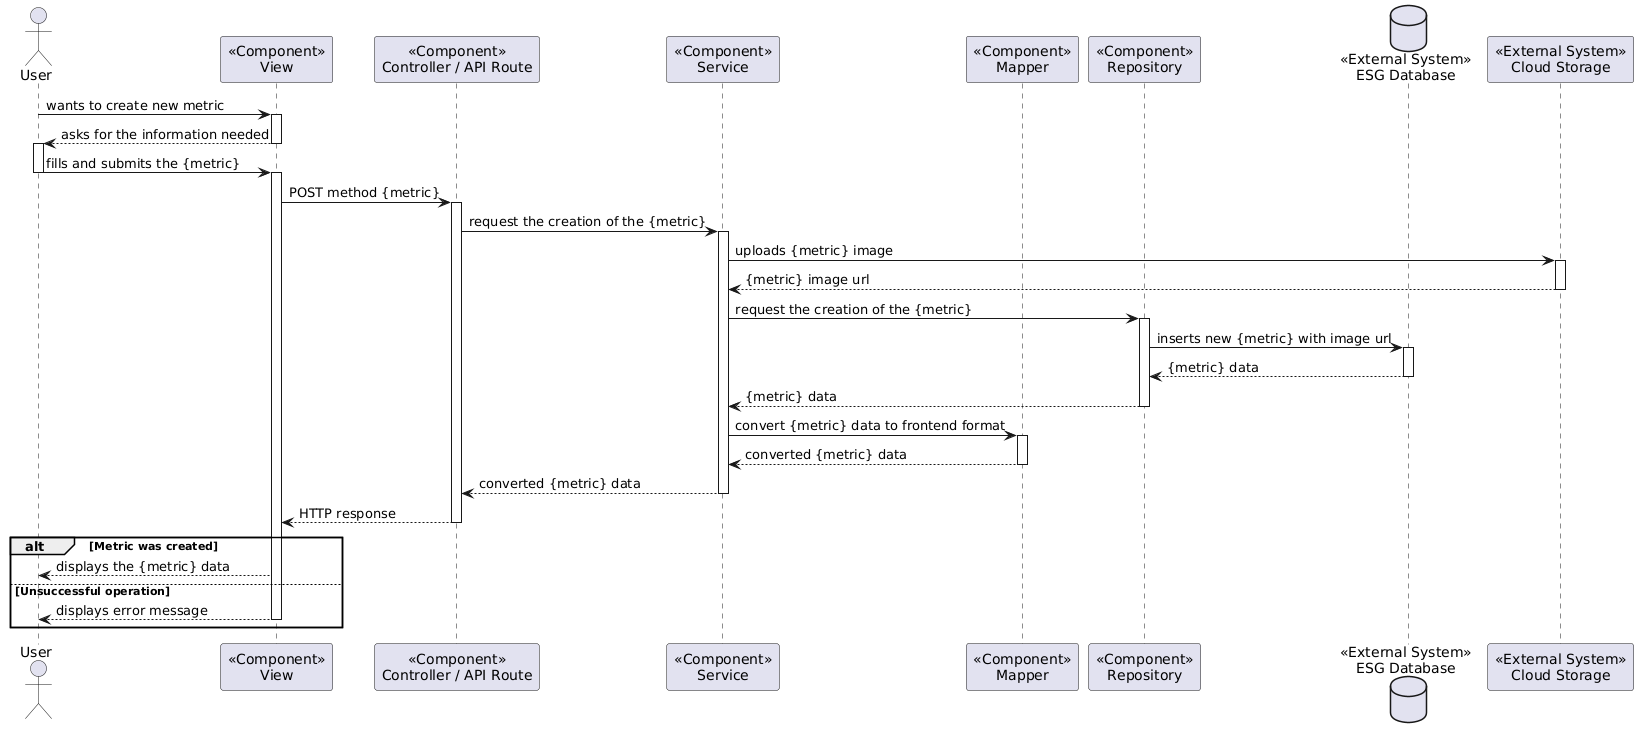
\includegraphics[width=\linewidth]{frontmatter/assets/diagrams/Process Views/LVL3/uc-06-lvl3.png}
\caption{Vista de processo do caso de uso de criação de métricas (Nível 3) (autoria própria)}
\label{fig:UC6-lvl3}
\end{figure}

De forma semelhante, o caso de uso UC-07 também apresenta essa distinção, evidenciada na Figura \ref{fig:UC7-lvl3}.

\begin{figure}[H]
\centering
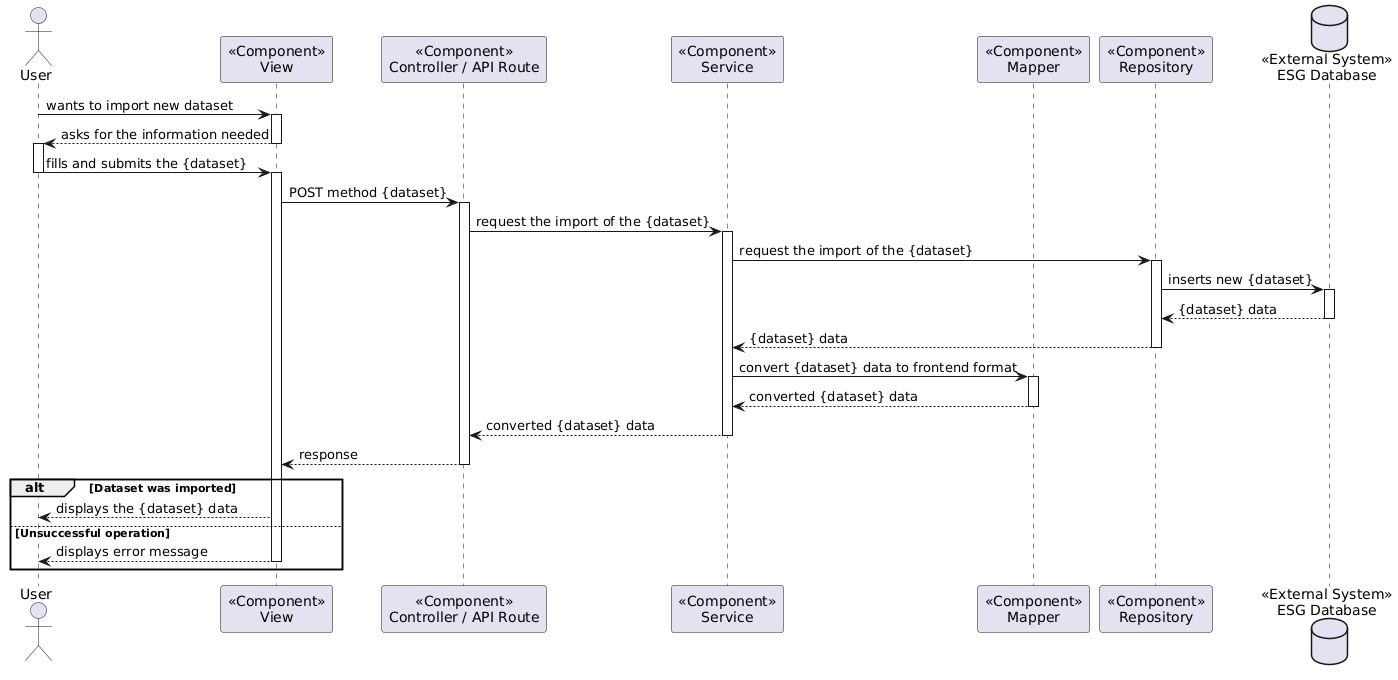
\includegraphics[width=\linewidth]{frontmatter/assets/diagrams/Process Views/LVL3/uc-07-lvl3.png}
\caption{Vista de processo dos casos de uso de importação de dados (Nível 3) (autoria própria)}
\label{fig:UC7-lvl3}
\end{figure}


\subsection{Vista de Cenários}

A vista de cenários, ilustrada pela Figura \ref{fig:scenario_view} e apresentada na secção \ref{subsec:FunReq}, compila os caso de usos principais. Esta vista é redundante, daí o "+1" na designação do modelo arquitetural (\cite{Kruchten1995}).

\subsection{Vista Lógica}

Esta vista será abordada por vários diagramas correspondentes a sucessivos níveis de detalhe na representação logica do sistema, iniciando-se pelo Nível 1, com a Figura \ref{fig:logical_view_lv1}, que permite entender o que o sistema disponibiliza, assim como que APIs consome.

\begin{figure}[H]
    \centering
    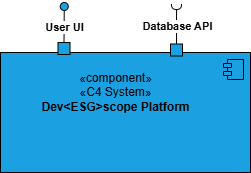
\includegraphics[width=3in,keepaspectratio]{frontmatter/assets/diagrams/Logical View/Logical View Lv1.drawio.png}
    \caption{Vista Lógica (Nível 1) (autoria própria)}
    \label{fig:logical_view_lv1}
\end{figure}

A Figura \ref{fig:logical_view_lv2} apresenta o Nível 2, oferecendo uma visão mais detalhada do sistema. Este nível inclui o contentor \textit{Frontend}, responsável por disponibilizar a \textit{User \gls{UI}}, através da qual os utilizadores interagem com a aplicação. Este contentor consome duas APIs, a \textit{Database API} e a \textit{Cloud Storage API}, que, respetivamente, comunicam com a base de dados e com o serviço de armazenamento na nuvem.

\begin{figure}[H]
    \centering
    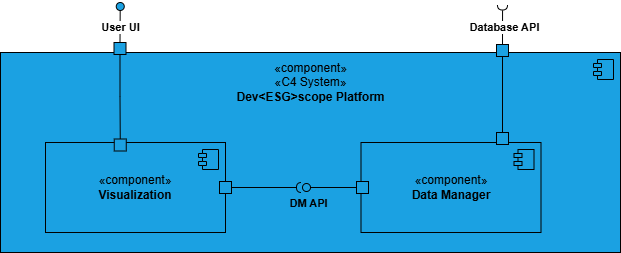
\includegraphics[width=4in,keepaspectratio]{frontmatter/assets/diagrams/Logical View/Logical View Lv2.drawio.png}
    \caption{Vista Lógica (Nível 2) (autoria própria)}
    \label{fig:logical_view_lv2}
\end{figure}

Já o Nível 3 (Figura \ref{fig:logical_view_lv3}) representa os componentes que compõem os contentores do sistema, tornando mais claras as interações entre eles.

Observa-se que o contentor \textit{Frontend} consome duas APIs: uma disponibilizada pelo \textit{Database Provider} e outra pelo \textit{Cloud Storage Provider}.

O \textit{Cloud Storage Provider} é utilizado para armazenar ficheiros estáticos (como imagens) e gerar os seus \textit{\gls{URL}} de acesso público. Estes URLs são posteriormente armazenados na base de dados.

O \textit{Database Provider}, por sua vez, utiliza uma base de dados relacional. A responsabilidade de persistir os dados, incluindo os URLs gerados, cabe ao contentor \textit{Frontend}, que interage diretamente com ambas as APIs.

\begin{landscape}
\begin{figure}[p]
    \centering
    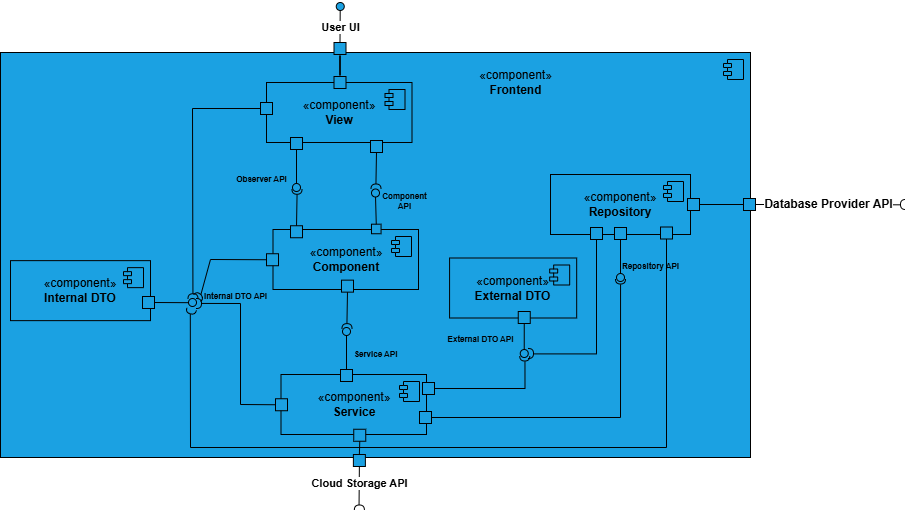
\includegraphics[width=\linewidth,keepaspectratio]{frontmatter/assets/diagrams/Logical View/Logical View Lv3.drawio.png}
    \caption{Vista Lógica (Nível 3) (autoria própria)}
    \label{fig:logical_view_lv3}
\end{figure}
\end{landscape}

\subsection{Vista de Implementação}

Semelhante à subsecção anterior, esta vista será detalhada somente com um diagrama de Nível 3, representado pela Figura \ref{fig:development_view_lv3}.

O Nível 1 não consta neste relatório por se tratar de uma representação demasiado abstrata, que pouco acrescentaria ao entendimento do sistema em questão. O Nível 2 não oferece nenhuma informação acrescida comparativamente ao diagrama do mesmo nível da vista lógica (Figura \ref{fig:logical_view_lv2}).

O Nível 3, de granularidade mais fina, elabora conteúdo do módulo \textit{Frontend}, dando um maior  entendimento não só na sua constituição mas também nas diferentes interações entre os seus elementos 

A aplicação Plataforma ESG é constituida por uma \textit{React \gls{SPA}} para o \textit{Frontend}, construída para suportar a geração atual de \textit{browsers} para \textit{desktop}.

Todas as ações realizadas pelos utilizadores têm origem no \textit{Frontend}, que comunica com o \textit{Database Provider} para obter ou inserir os dados necessários. No caso específico da criação de uma nova métrica, o \textit{Frontend} interage adicionalmente com o \textit{Cloud Storage Provider}, onde ocorre o \textit{upload} da imagem representativa da respetiva métrica.

\begin{figure}[H]
    \centering
    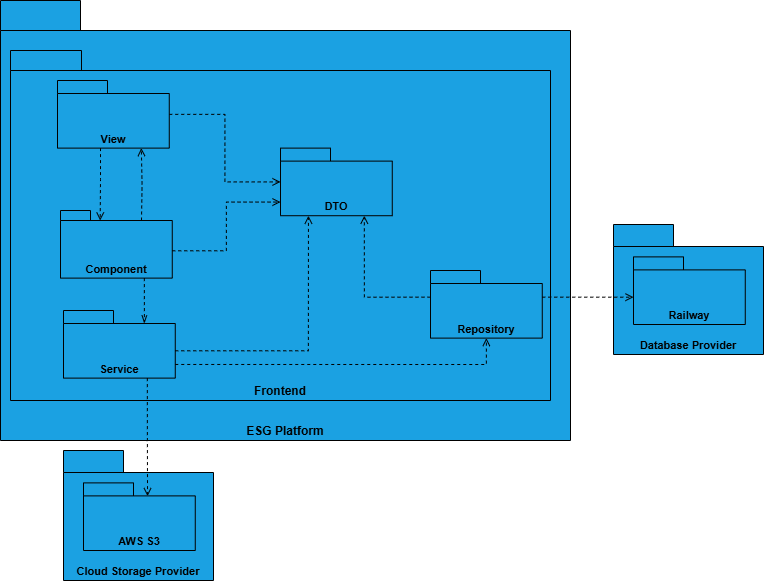
\includegraphics[width=4.75in,keepaspectratio]{frontmatter/assets/diagrams/Development View/Implementation Lv3.drawio.png}
    \caption{Vista de Implementação (Nível 3) (autoria própria)}
    \label{fig:development_view_lv3}
\end{figure}

O Apêndice \ref{AppendixB} apresenta o mapeamento entre a vista lógica e a de implementação de Nível 3 de modo a facilitar o entendimento das relações entre as duas vistas.
    
\subsection{Vista Física}

A vista física tem como objetivo mapear o \textit{software} para o \textit{hardware}, com ênfase nos requisitos não funcionais do sistema, como disponibilidade,confiabilidade (tolerância a falhas), desempenho e escalabilidade (\cite{Kruchten1995}). A Figura \ref{fig:physical_view_lv2} apresenta o diagrama de Nível 2 da vista física da solução desenvolvida.

\begin{figure}[H]
    \centering
    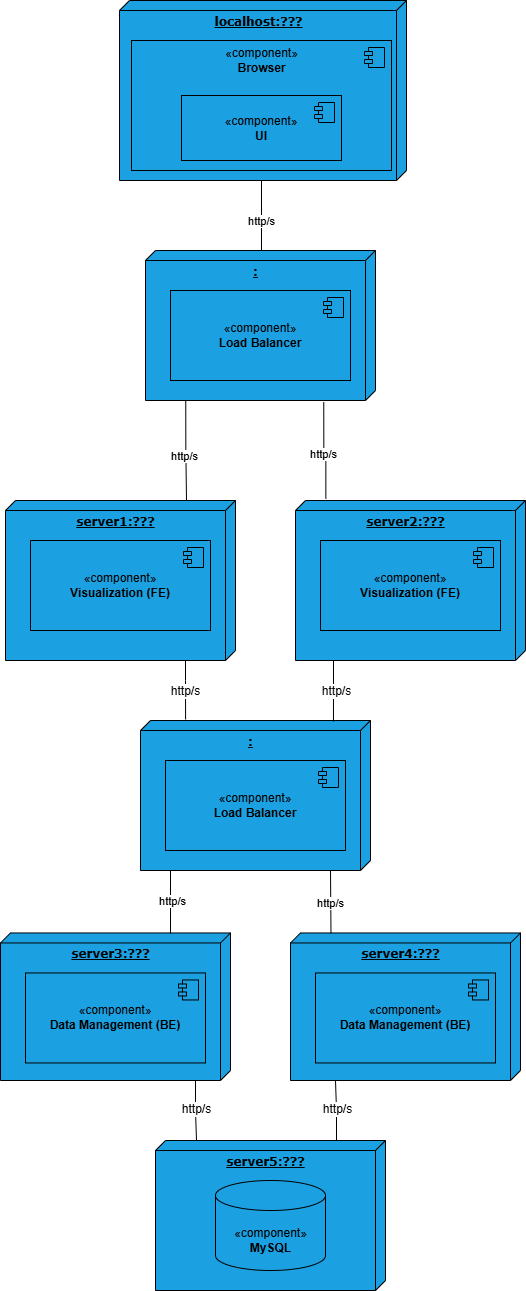
\includegraphics[height=5.75in,keepaspectratio]{frontmatter/assets/diagrams/Physical View/physical_view_lv2.drawio.png}
    \caption{Diagrama de Nível 2 da vista física da solução (autoria própria)}
    \label{fig:physical_view_lv2}
\end{figure}

Os \textit{Load Balancers} são responsáveis por distribuir o tráfego de forma dinâmica entre os servidores que compõem as camadas de \textit{Frontend} e \textit{Data Management} (\textit{backend} com base de dados). Estes atuam como intermediários entre os utilizadores e os servidores, assegurando uma distribuição equilibrada da carga, especialmente durante períodos de maior tráfego. Com isso, aumentam a disponibilidade e a resiliência do sistema: caso um servidor falhe, o tráfego é automaticamente redirecionado para outro servidor ativo (tolerância a falhas). Esta abordagem contribui ainda para a redução da latência e para evitar respostas inconsistentes da aplicação (\Cite{F52025}).

As comunicações entre os vários componentes são realizadas através de protocolo HTTP ou HTTPS.

\section{Alternativa Arquitetural: DDD com \textit{Clean Architecture}}
\label{sec:SolAlt}

Uma alternativa à arquitetura representada pelos modelos C4/4+1 seria o uso de \textit{Domain-Driven Design} (DDD) combinado com os princípios da \textit{Clean Architecture}. Esta abordagem também permite uma estrutura modular e escalável, alinhada aos limites naturais do domínio e preparada para futuras expansões.

Como mostra a Figura \ref{fig:alternativeModel}, o sistema é dividido em módulos independentes, cada um representando um conceito central da aplicação ESG: \textit{Dataset}, \textit{Metric}, \textit{Objective}, \textit{Pillar} e \textit{Subarea}. Cada módulo encapsula as suas entidades, regras de negócio e casos de uso, comunicando-se com o exterior por meio de interfaces (\textit{ports}), enquanto os adaptadores (como base de dados ou APIs) implementam essas interfaces.

A estrutura segue o modelo em anéis concêntricos da \textit{Clean Architecture}, isolando o núcleo de domínio das dependências externas. Os casos de uso coordenam a lógica na camada de aplicação, e as camadas mais externas lidam com \textit{frameworks} como \textit{Prisma} ou \textit{Next.js}.

Esta organização garante separação clara de responsabilidades, menor acoplamento, maior testabilidade e independência tecnológica. Estes são fatores que contribuem para um código mais limpo, coeso e sustentável.

\begin{figure}[H]
    \centering
    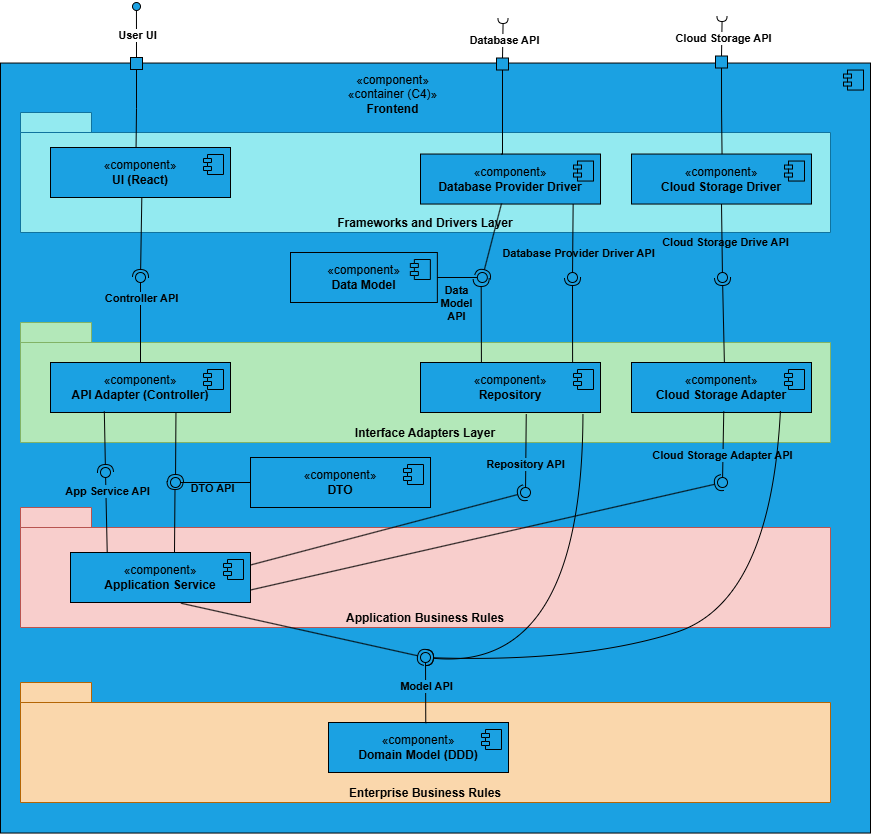
\includegraphics[height=5in,keepaspectratio]{frontmatter/assets/diagrams/AlternativeModel.drawio.png}
    \caption{Diagrama de Nível 3 da vista lógica do \textit{container Frontend} segundo uma arquitetura de camadas concêntricas (autoria própria)}
    \label{fig:alternativeModel}
\end{figure}
% % 
\chapter{Implementação da Solução} 
\label{chap:Impl} % For referencing the chapter elsewhere, use Chapter~\ref{Impl}

Este capítulo deve ser dedicado à apresentação de detalhes relacionados com o enquadramento e implementação das soluções preconizadas no capítulo anterior. Note-se, no entanto, que detalhes desnecessários à compreensão do trabalho devem ser remetidos para anexos. Dependendo do volume, a avaliação do trabalho pode ser incluída neste capítulo ou pode constituir um capítulo separado.

%-------------------------------------------------------------------------------

\section{Descrição da implementação} 
\label{sec:desc} %For referencing this section elsewhere, use Section~\ref{sec:desc}

Descrever a implementação da solução proposta no capítulo anterior, podendo ser dadas explicações e evidências de soluções intercalares. Devem também ser descritas as tecnologias e metodologias utilizadas (software, sistemas de operação, linguagens, dispositivos ou outras ferramentas) e perspetiva crítica sobre as mesmas. 

Esta secção descreve a implementação da solução proposta no capítulo anterior. 

Alguns dos diagramas referidos na secção anterior podem aparecer nesta secção. Por exemplo, diagramas de classes ou diagramas de módulos, sendo detalhadas as operações de cada classe ou as funções de cada módulo (diagramas de atividades). 

Devem também ser descritas as especificidades de implementação de acordo com o ambiente de desenvolvimento, plataforma e linguagem escolhida para o desenvolvimento e deve ser claro que o desenho apresentado anteriormente foi, de facto, adotado na implementação

\textbf{Descrição da fase de implementação no processo de Engenharia de Software}

\subsection{Tecnologias Usadas}

\textbf{Menção da divisão das tecnologias em duas categorias: pré-desenvolvimento e desenvolvimento}

\subsubsection{Tecnologias de Pré-desenvolvimento}

- Plantuml \\
- VSCode \\
- Draw.io \\
- Figma (anexo com imagens dos mockups) \\
- Github Projects (mostrar setup do projecto e dos cartões) + Repository \\

Site do \textit{Figma}: \url{https://www.figma.com/} \\
Site do \textit{Github}: \url{https://github.com/} \\
Site do \textit{Draw\.io}: \url{https://www.drawio.com/} \\
Site do \textit{Plantuml}: \url{https://plantuml.com/} \\
Site do \textit{Visual Studio Code}: \url{https://code.visualstudio.com/} \\


\subsubsection{Tecnologias de Desenvolvimento}

- Visual Studio Code \\
- React \\
- Next.js \\
- Tailwind CSS \\
- http requests \\
- Vuexy template \\
- AWS S3 \\
- Prisma
- Railway com MySQL database \\


Site do \textit{React}: \url{https://react.dev/} \\
Site do \textit{Next.js}: \url{https://nextjs.org/} \\
Site do \textit{Tailwind CSS}: \url{https://tailwindcss.com/} \\
Site do \textit{Vuexy}: \url{https://pixinvent.com/vuexy-bootstrap-html-admin-template/} \\
Site do \textit{AWS S3}: \url{https://aws.amazon.com/s3/} \\
Site do \textit{Prisma}: \url{https://www.prisma.io/} \\
Site do \textit{Railway}: \url{https://railway.com/} \\


\section{Funcionalidades}

\subsection{Home Page | \textit{Dashboard}}

- KPIs \\
- ESG Score (+ formula) \\
- Best metrics since last record \\
- Worse metrics since last record \\

\subsection{Página das Métricas}

- Display \\
- Cards \\
- Filtering \\
- Creation of Metrics \\

\subsection{Mapa de Materialidade}

- Mapa Display \\
metion that when clicked it will open a generic metric card

\subsection{Página dos Datasets}

- Display \\
- Card \\
- Show Filtering \\
- Show import \\
- Show deletion (maybe) \\

\subsection{Página dos Objetivos}

mention its a complementary part tha the company showed interest in implementing

- Display \\
- Creation of objectives \\

\section{Testes} 

- Teste unitarios aos componentes
- Alguns de integraçao

mostrar apenas print das cenas a passarem + 1 exemplo de unitario, 1 exemplo de integraçao

(maybe E2E ???)

A descrição dos testes efetuados (e.g. unitários, funcionais, de integração, de sistema) pode ser feita nesta secção ou, caso não se justifique, na secção anterior.

\section{Avaliação da solução} 

Nesta secção deve ser descrita a abordagem seguida para avaliar a solução, ou parte da solução, nomeadamente um ou mais requisitos de qualidade (e.g. desempenho, usabilidade). 

São descritas experiências efetuadas e apresentados os dados/modelos utilizados, bem como os resultados obtidos. 

Devem ser descritos e avaliados os resultados obtidos. 

Deve ser feita uma discussão sobre a adequação dos resultados obtidos relativamente aos planeados anteriormente. 

Esta secção poderá não existir em alguns relatórios de projeto/estágio, mas nesse caso deverá ser dada uma justificação para tal. 

% \input{chapters/Conclusões}

%----------------------------------------------------------------------------------------
%	BIBLIOGRAPHY
%----------------------------------------------------------------------------------------

\printbibliography[heading=bibintoc]

%----------------------------------------------------------------------------------------
%	THESIS CONTENT - APPENDICES
%----------------------------------------------------------------------------------------

\appendix % Cue to tell LaTeX that the following "chapters" are Appendices

% Include the appendices of the thesis as separate files from the Appendices folder
% Uncomment the lines as you write the Appendices

% \chapter{Cronograma do Projeto de Estágio}
\label{AppendixA}

O presente gráfico de Gantt apresenta o cronograma do projeto de estágio, detalhando as fases e prazos das atividades planeadas.

\begin{figure}[h]
    \centering
    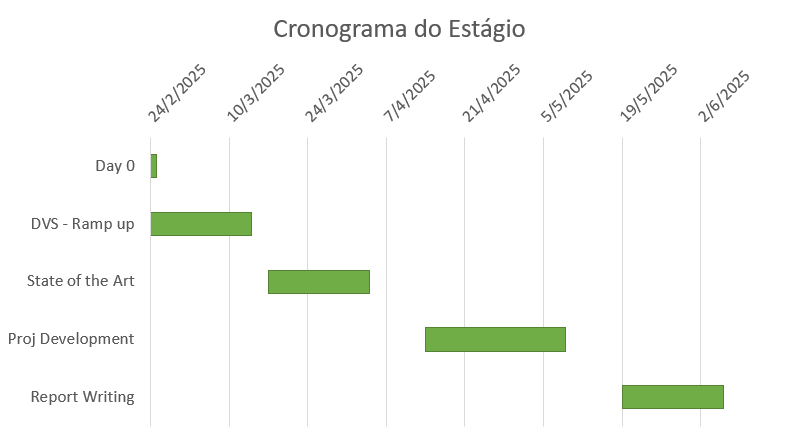
\includegraphics[width=\linewidth]{/frontmatter/assets/cronograma.png}
    \caption{Cronograma do projeto de estágio}
    \label{fig:cronograma}
\end{figure}
%\chapter{Mapeamento entre vistas de Implementação e Lógica (Nível 3)}
\label{AppendixB}

\begin{figure}[h]
    \centering
    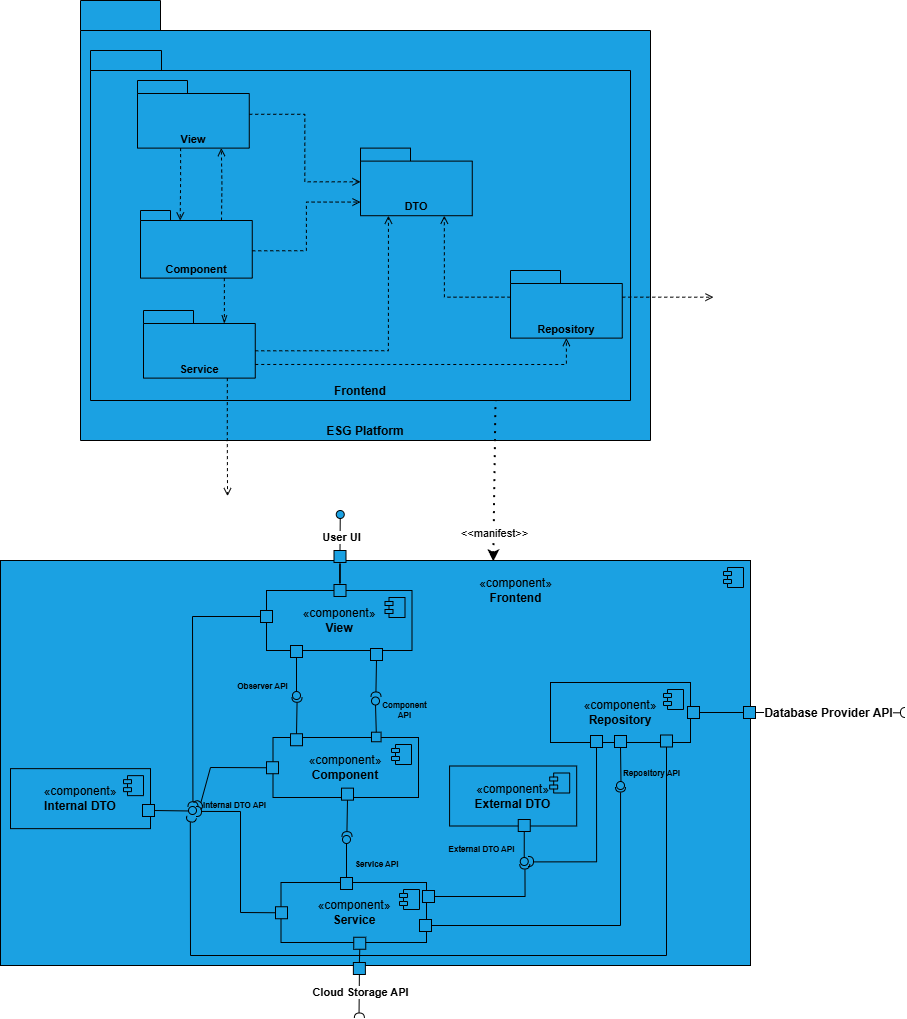
\includegraphics[width=5in]{frontmatter/assets/diagrams/Mapeamento.drawio.png}
    \caption{Mapeamento entre vistas de Implementação e Lógica (Nível 3)}
    \label{fig:mapeamento}
\end{figure}
%\chapter{\textit{Designs} do \textit{Figma}}
\label{AppendixC}

O seguinte Apêndice apresenta os \textit{designs} do \textit{mockup}  desenvolvido na plataforma Figma para o projeto em questão. A criação deste protótipo surgiu da ênfase dada à área de \textit{Frontend} durante o estágio, sendo a idealização da interface e a organização da informação elementos fundamentais para um desenvolvimento mais ágil, coerente e orientado.

O objetivo principal do \textit{mockup} foi validar a arquitetura de informação, a experiência do utilizador e a adequação visual da plataforma às necessidades da empresa.

O protótipo serviu como base de referência para a implementação da interface, reduzindo ambiguidades e acelerando o processo de desenvolvimento ao fornecer uma visão clara das funcionalidades e do seu comportamento esperado. Este foi submetido à empresa, que o aprovou e forneceu um \textit{feedback} positivo, validando as decisões de \textit{design} tomadas.

As imagens seguintes ilustram algumas das páginas principais do protótipo, incluindo o painel de controlo, a personalização de métricas e a criação de objetivos.

\begin{figure}[H]
\centering
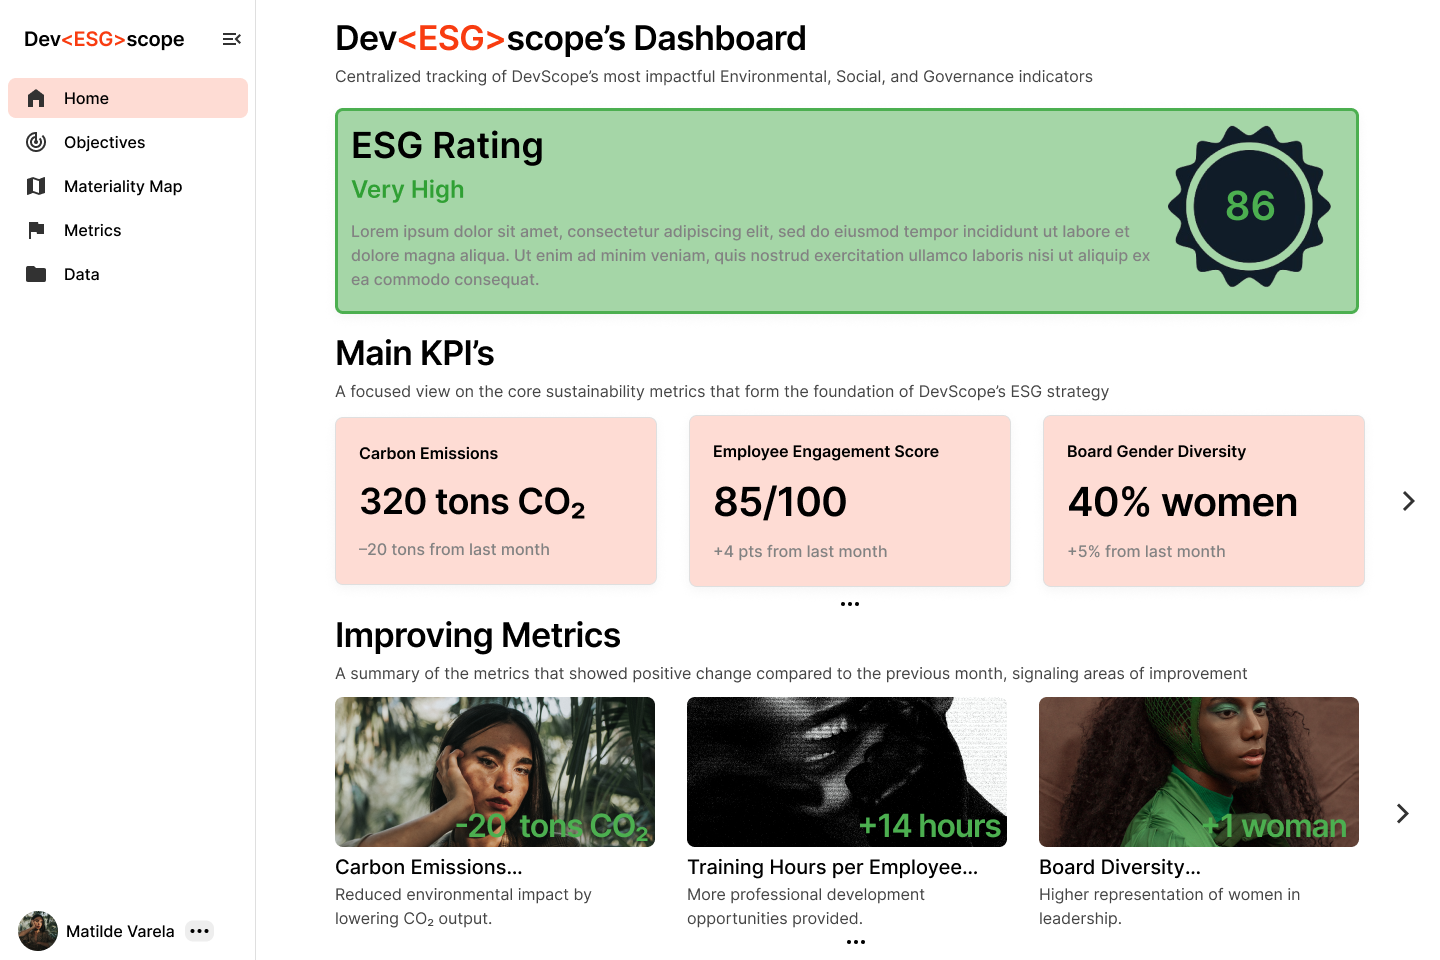
\includegraphics[width=\linewidth]{/frontmatter/assets/mockup/Dashboard _ Home Page.png}
\captionof{figure}{Página Inicial (Dashboard) da Plataforma ESG}
    \label{fig:dashboardESG}
\end{figure}

%-----------------------------------------------------------

\begin{landscape}
\centering
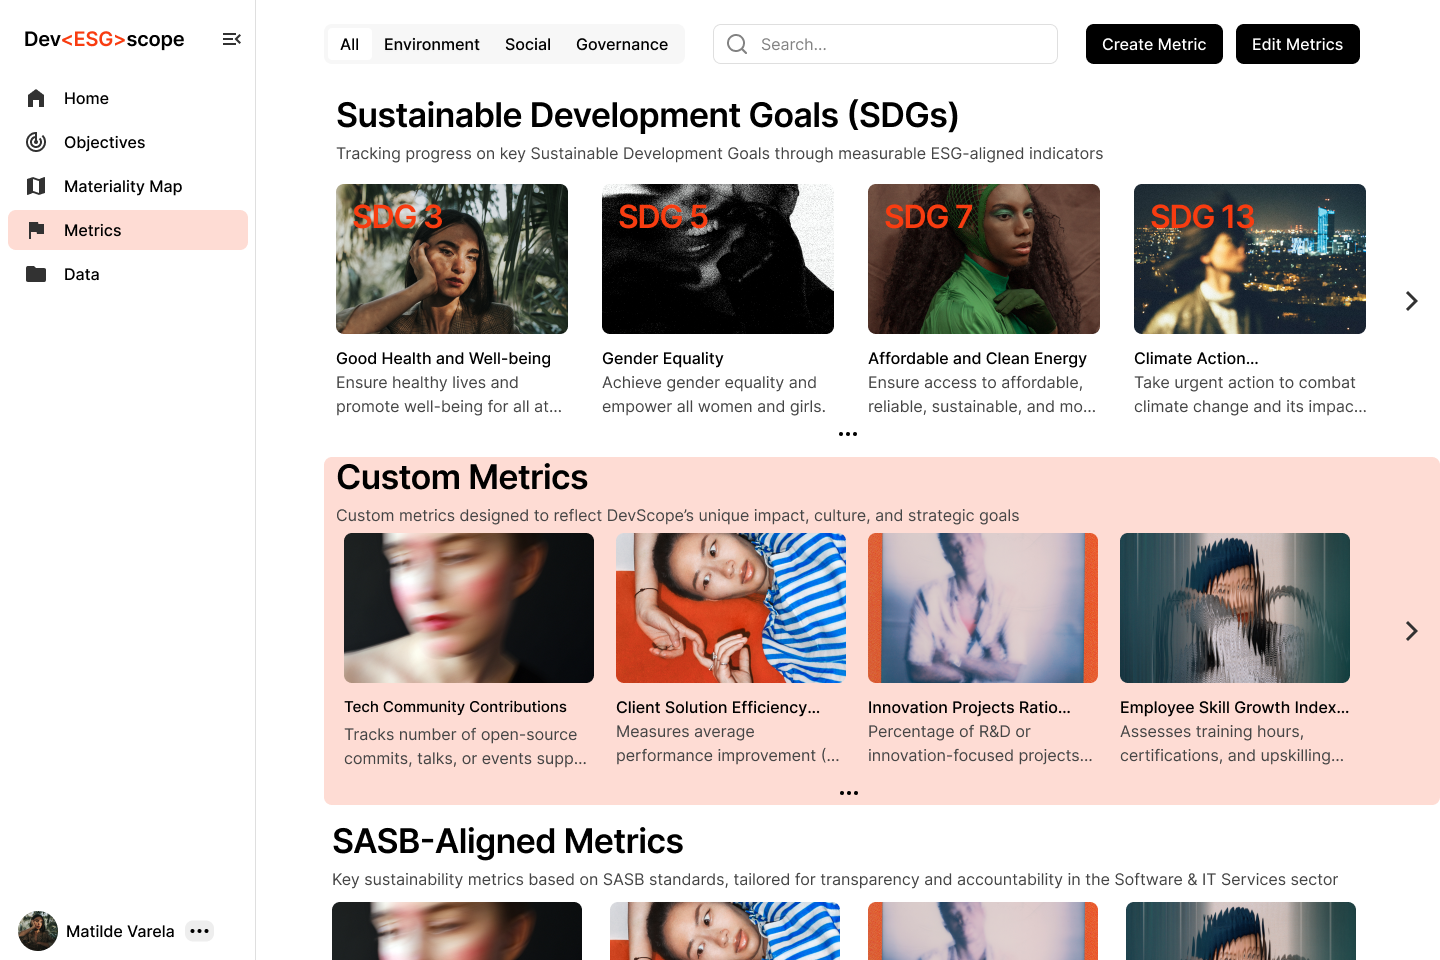
\includegraphics[width=0.9\linewidth]{frontmatter/assets/mockup/Metrics_and_ODS_Customization.png}
\captionof{figure}{Página das Métricas Customizáveis e de SASB (autoria própria)}
\label{fig:metricPage}
\end{landscape}


\begin{figure}[H]
    \centering
    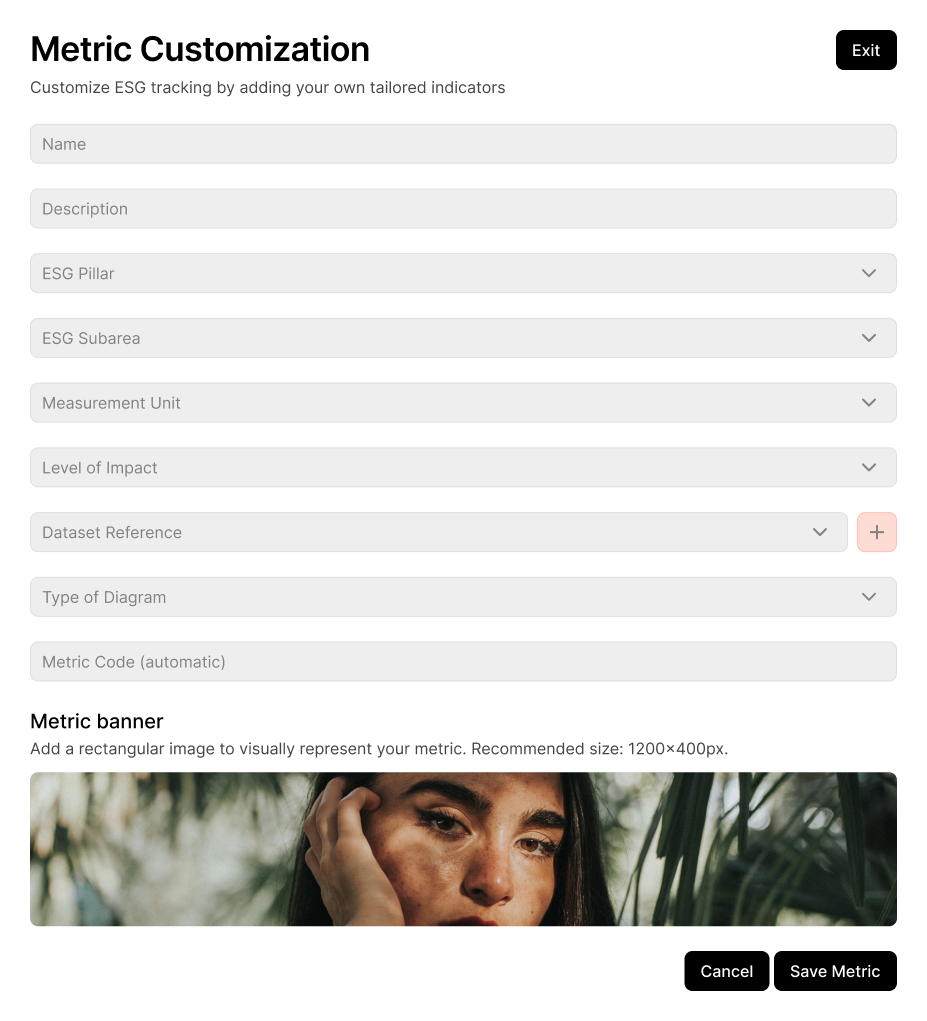
\includegraphics[width=\linewidth]{frontmatter/assets/mockup/Custom Metric Creation.png}
    \caption{Painel de Criação de Métricas Customizáveis (autoria própria)}
    \label{fig:customMetricModal}
\end{figure}


\begin{figure}[H]
    \centering
    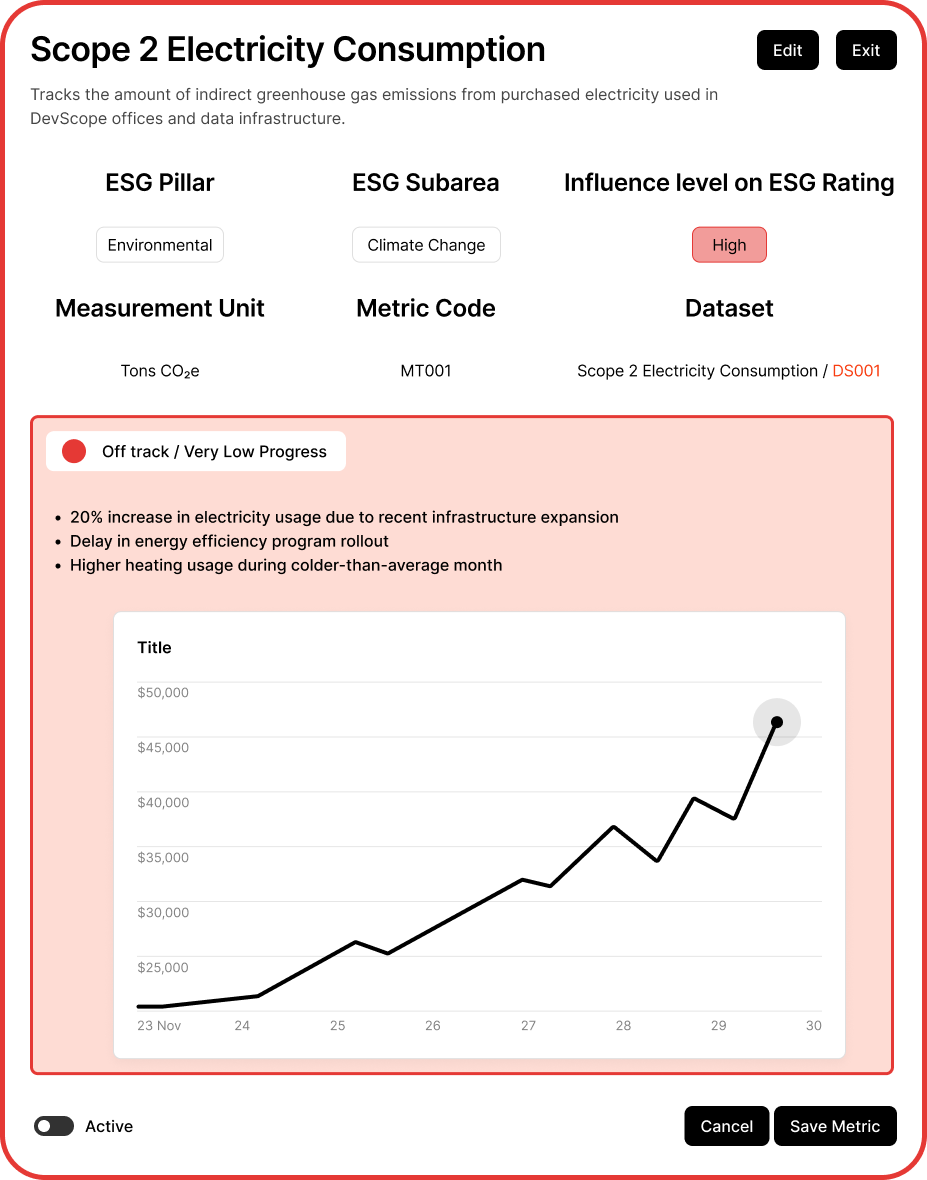
\includegraphics[width=\linewidth]{frontmatter/assets/mockup/Metric Card.png}
    \caption{Painel de Informação da Métrica (autoria própria)}
    \label{fig:metricInfoModal}
\end{figure}

%-----------------------------------------------------------

\begin{figure}[H]
    \centering
    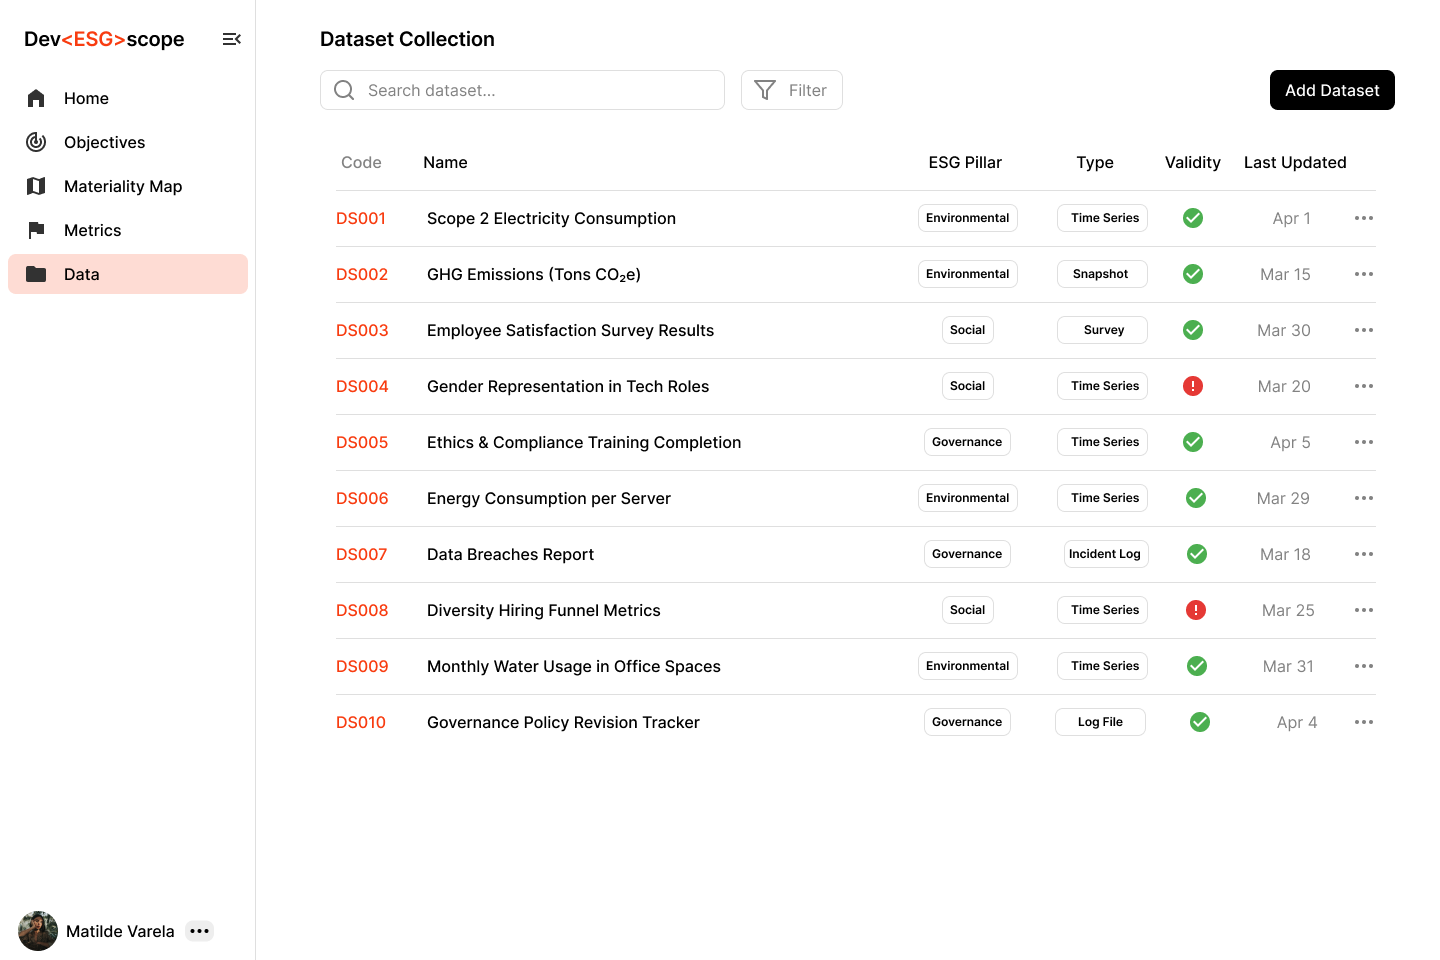
\includegraphics[width=\linewidth]{frontmatter/assets/mockup/Data Collection Database.png}
    \caption{Página dos Conjuntos de Dados (autoria própria)}
    \label{fig:datasetPage}
\end{figure}

\begin{figure}[H]
    \centering
    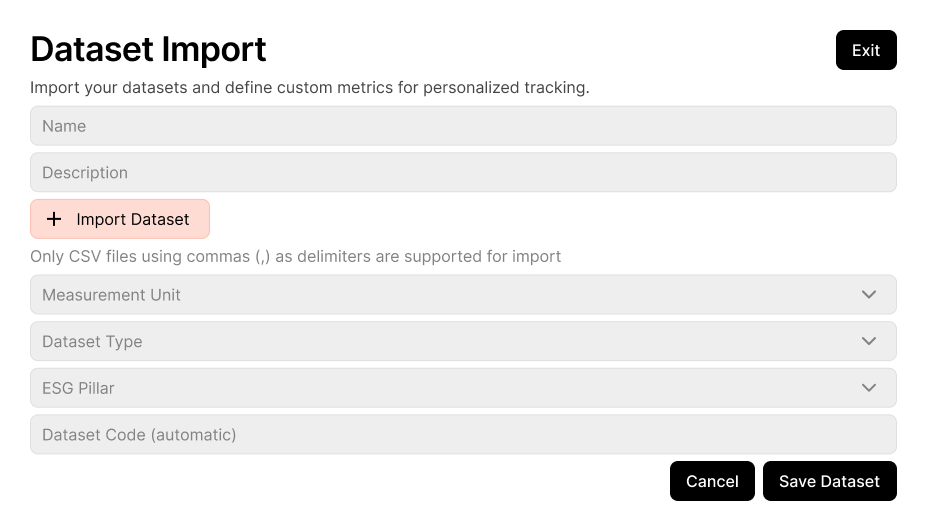
\includegraphics[width=\linewidth]{frontmatter/assets/mockup/Data Import.png}
    \caption{Painel de Importação de Conjuntos de Dados (autoria própria)}
    \label{fig:importDatasetModal}
\end{figure}

%-----------------------------------------------------------

\begin{figure}[H]
    \centering
    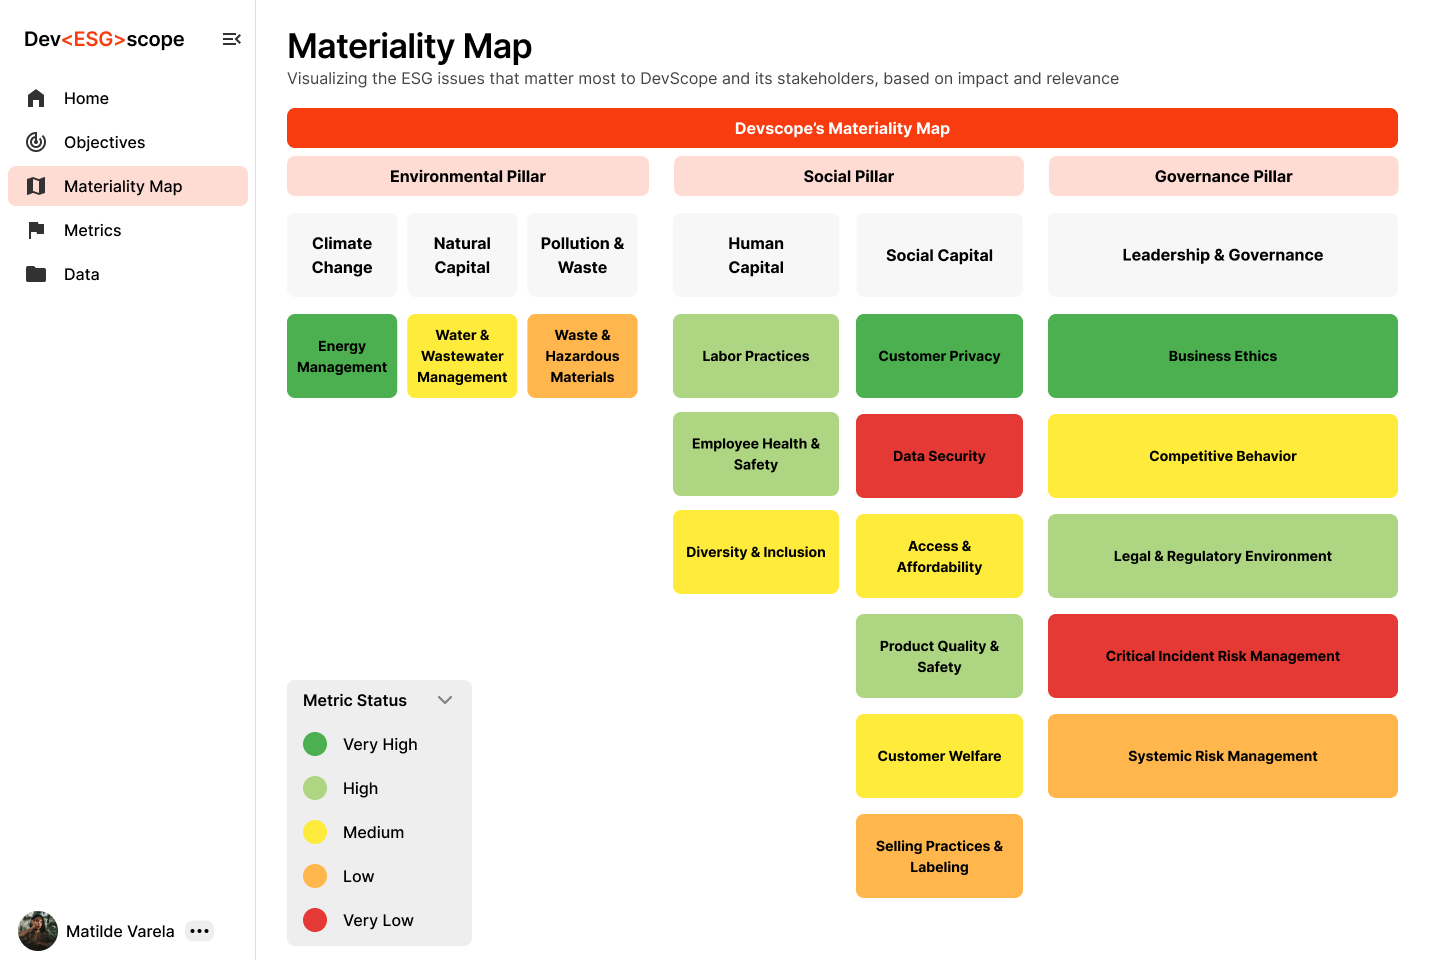
\includegraphics[width=\linewidth]{frontmatter/assets/mockup/Matrix.png}
    \caption{Matriz de Materialidade segundo o setor de \textit{Software} e Serviços IT da \gls{SASB} (autoria própria)}
    \label{fig:matrixPage}
\end{figure}

%-----------------------------------------------------------

\begin{figure}[H]
    \centering
    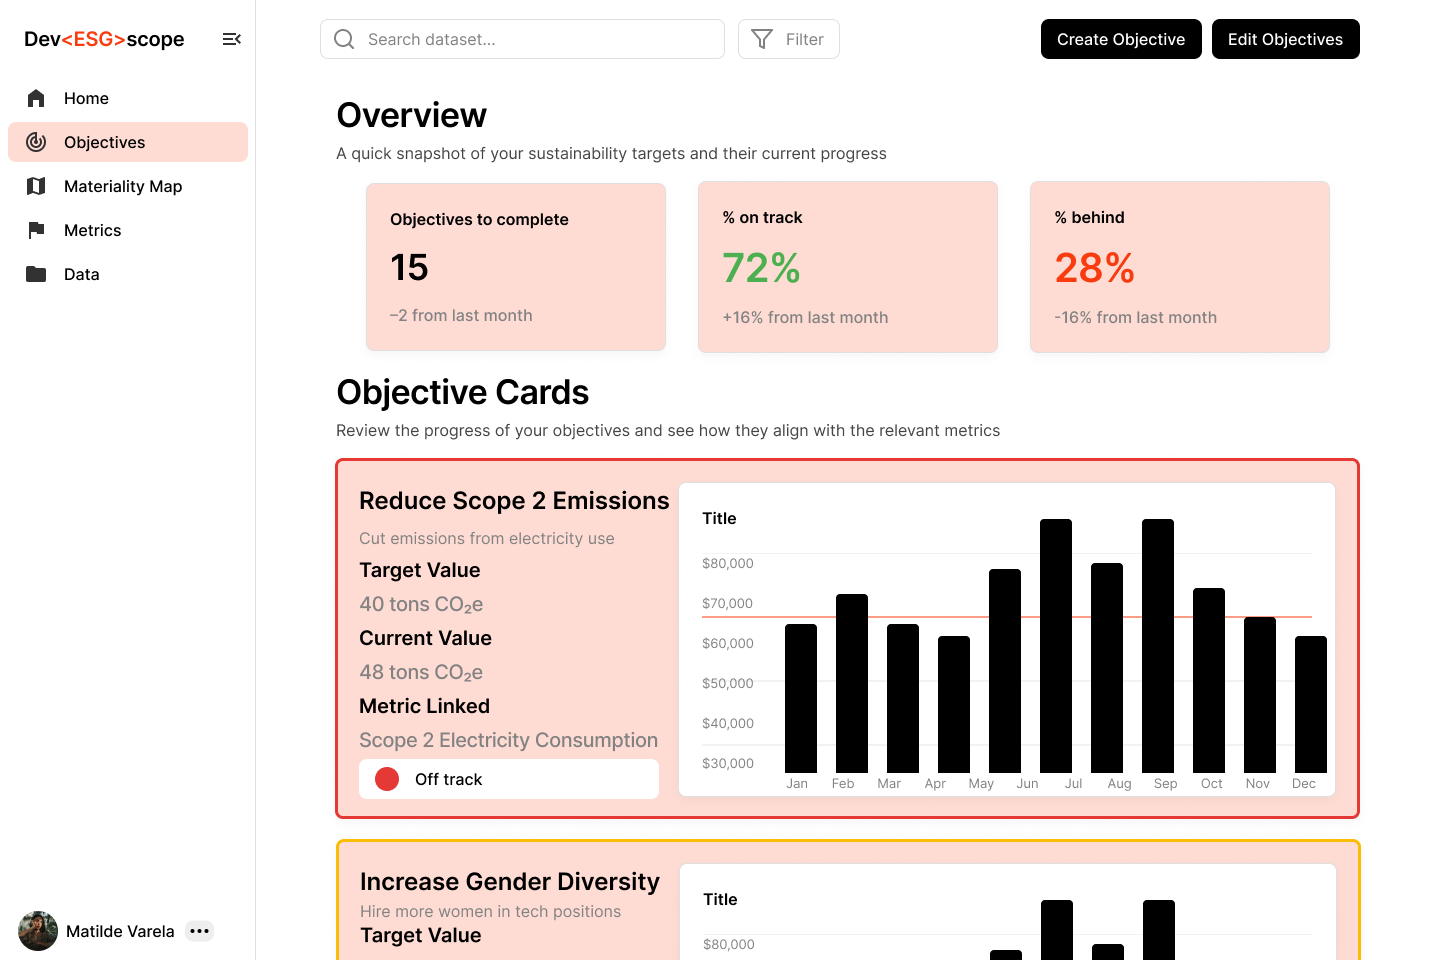
\includegraphics[width=\linewidth]{frontmatter/assets/mockup/Objective Tracking + Comparision with current Metrics.png}
    \caption{Página dos Objetivos (autoria própria)}
    \label{fig:objectivePage}
\end{figure}

\begin{figure}[H]
    \centering
    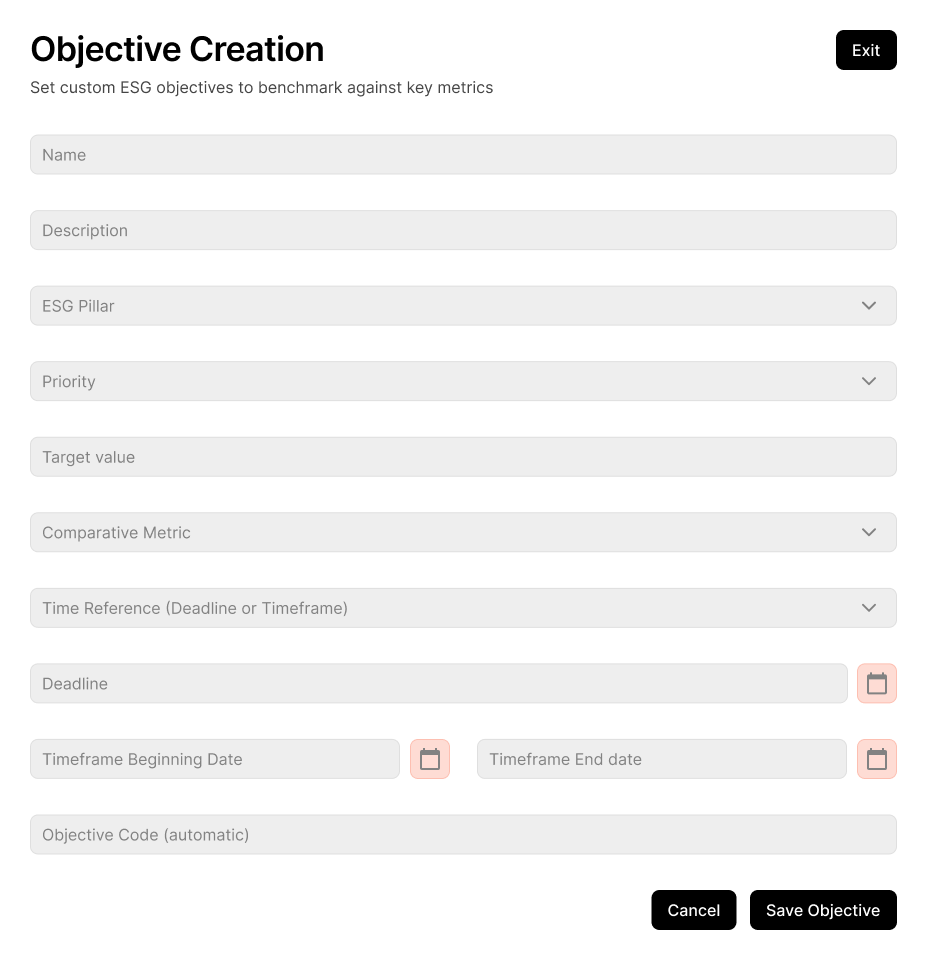
\includegraphics[width=\linewidth]{frontmatter/assets/mockup/Objective Creation.png}
    \caption{Painel de Criação de Objetivos (autoria própria)}
    \label{fig:customObjectiveModal}
\end{figure}

%----------------------------------------------------------------------------------------

\end{document}